% !TeX program = xelatex
% !TeX encoding = UTF-8
% Presentazione revisionata: Strata · Cronologie e archivi sedimentari
% Basata sul materiale originale fornito dall'autore e sul template M01_Pensare_con_i_dati.tex
% Compilazione: xelatex -interaction=nonstopmode M13_Strata.tex (due passaggi)
% Diagrammi TikZ e figure statistiche vettoriali; sorgenti R e dati inclusi.
% 63 slide. Materiali R6 e impaginazione della serie planetaria.
\RequirePackage{fix-cm}
\documentclass[12pt,aspectratio=1610]{beamer}
\geometry{paperwidth=20cm,paperheight=12.5cm}
\usepackage[italian,provide=*]{babel}
\usepackage{fontspec,adjustbox,tabularx}
\IfFontExistsTF{NimbusSans-Regular.otf}{
\setsansfont{NimbusSans-Regular.otf}[BoldFont=NimbusSans-Bold.otf,ItalicFont=NimbusSans-Italic.otf,BoldItalicFont=NimbusSans-BoldItalic.otf]
\setmainfont{NimbusSans-Regular.otf}[BoldFont=NimbusSans-Bold.otf,ItalicFont=NimbusSans-Italic.otf,BoldItalicFont=NimbusSans-BoldItalic.otf]
}{
\setsansfont{TeX Gyre Heros}
\setmainfont{TeX Gyre Heros}
}
\IfFontExistsTF{DejaVu Sans Mono}{
\setmonofont{DejaVu Sans Mono}[Scale=.88]
}{\setmonofont{Latin Modern Mono}[Scale=.88]}
\usefonttheme{professionalfonts}
\usepackage{amsmath,amssymb,booktabs,array,graphicx,tikz,bookmark}
\usetikzlibrary{calc,positioning,arrows.meta}
\graphicspath{{Figure/}}
\definecolor{Paper}{HTML}{F8F6F1}
\definecolor{Ink}{HTML}{253344}
\definecolor{Navy}{HTML}{15283E}
\definecolor{Quantum}{HTML}{5146A5}
\definecolor{Classical}{HTML}{087C74}
\definecolor{Muted}{HTML}{657180}
\definecolor{Rule}{HTML}{D6DAD9}
\definecolor{Night}{HTML}{112236}
\definecolor{Lilac}{HTML}{ABB5FF}
\definecolor{Mint}{HTML}{72D8C8}
\setbeamercolor{background canvas}{bg=Paper}
\setbeamercolor{normal text}{fg=Ink}
\setbeamertemplate{navigation symbols}{}
\setbeamertemplate{headline}{}
\setbeamertemplate{footline}{}
\setbeamersize{text margin left=0pt,text margin right=0pt}
\hypersetup{colorlinks=true,linkcolor=Classical,urlcolor=Classical,pdfpagemode=UseOutlines,pdfstartview=Fit,
 pdftitle={Strata · Cronologie e archivi sedimentari},pdfauthor={GeoStat Lab · materiali di Marzio De Corato},
 pdfsubject={GeoStat Lab · M13}}
\bookmarksetup{open,openlevel=0,depth=2}
\newsavebox{\BodyBox}
\newsavebox{\SideBox}
\newsavebox{\RecallBox}
\newsavebox{\TitleBox}
\newcommand{\MeasureBox}[2]{\typeout{REVIEWBOX:#1:\the\wd#2:\the\ht#2:\the\dp#2}}

% Revisione completa: diagrammi TikZ, formalismo e box R.
\usepackage[most]{tcolorbox}
\usepackage{listings}
\usetikzlibrary{fit,backgrounds,matrix,decorations.pathreplacing}
\definecolor{GeoA}{HTML}{1D7890}
\definecolor{GeoB}{HTML}{C57E42}
\definecolor{GeoC}{HTML}{7363AA}
\definecolor{GeoTint}{HTML}{F0F4F3}
\lstdefinestyle{GeoR}{language=R,basicstyle=\ttfamily\fontsize{9.2}{12.2}\selectfont,
 keywordstyle=\color{Quantum}\bfseries,commentstyle=\color{Classical},stringstyle=\color{GeoB},
 numbers=left,numberstyle=\tiny\color{Muted},numbersep=4pt,showstringspaces=false,
 columns=fullflexible,keepspaces=true,breaklines=true,xleftmargin=1.15em,
 frame=none,aboveskip=0pt,belowskip=0pt,tabsize=2}
\newsavebox{\PilotLeftBox}
\newsavebox{\PilotRightBox}
\newcommand{\PLabel}[1]{\par{\color{Classical}\bfseries\fontsize{9}{11}\selectfont\MakeUppercase{#1}}\par\vspace{1.8mm}}
\newcommand{\PBody}[1]{\par{\fontsize{11.3}{14.8}\selectfont #1\par}}
\newcommand{\PSmall}[1]{\par{\fontsize{9.8}{13.1}\selectfont #1\par}}
\newcommand{\PCode}[2]{%
\begin{tcolorbox}[enhanced,arc=1.8mm,boxrule=.65pt,
  colback=white,colframe=Classical!75!Navy,colbacktitle=Navy,
  coltitle=white,fonttitle=\bfseries\fontsize{9.6}{12}\selectfont,
  title={#1},left=1.7mm,right=1.3mm,top=1.5mm,bottom=1.3mm,
  before skip=1mm,after skip=1mm]
\lstinputlisting[style=GeoR]{Codice/#2}
\end{tcolorbox}}
\newcommand{\PInfo}[1]{%
\begin{tcolorbox}[enhanced,arc=1.6mm,boxrule=.55pt,colback=GeoTint,
 colframe=Rule!80!Classical,left=2.3mm,right=2.3mm,top=2mm,bottom=2mm,
 before skip=1mm,after skip=1mm]
\PSmall{#1}\end{tcolorbox}}
\tikzset{
 pFlow/.style={draw=Classical!45,fill=white,rounded corners=2mm,
  line width=.7pt,align=center,minimum height=1.1cm,font=\sffamily\fontsize{10}{12}\selectfont},
 pEdge/.style={-{Latex[length=2.3mm]},draw=Classical,line width=.95pt},
 pGroup/.style={draw=Rule,fill=white,rounded corners=2mm,line width=.65pt},
 pDotA/.style={circle,fill=GeoA,inner sep=1.25pt},
 pDotB/.style={circle,fill=GeoB,inner sep=1.25pt},
 pDotC/.style={circle,fill=GeoC,inner sep=1.25pt}
}
\newcommand{\PilotChrome}[4]{%
  \node[anchor=north west,inner sep=0,text width=17.7cm] at ([xshift=.95cm,yshift=-.55cm]current page.north west) {\color{Navy}\bfseries\fontsize{20.6}{24.5}\selectfont #1};
  \node[anchor=north east,inner sep=0] at ([xshift=19.05cm,yshift=-.14cm]current page.north west) {\color{Classical}\fontsize{8}{10}\selectfont\hyperlink{slide2}{#2}};
  \draw[Classical,line width=1.2pt] ([xshift=.95cm,yshift=-1.7cm]current page.north west)--([xshift=2.35cm,yshift=-1.7cm]current page.north west);
  \draw[Rule,line width=.65pt] ([xshift=.95cm,yshift=-10.36cm]current page.north west)--([xshift=19.05cm,yshift=-10.36cm]current page.north west);
  \node[anchor=north west,inner sep=0] at ([xshift=.96cm,yshift=-10.55cm]current page.north west) {\color{Classical}\bfseries\fontsize{9.1}{12}\selectfont DA RICORDARE};
  \node[anchor=north west,inner sep=0,text width=14.3cm] at ([xshift=4.2cm,yshift=-10.53cm]current page.north west) {\color{Ink}\fontsize{10.3}{13.8}\selectfont #4};
  \draw[Rule,line width=.35pt] ([xshift=.95cm,yshift=-11.92cm]current page.north west)--([xshift=19.05cm,yshift=-11.92cm]current page.north west);
  \node[anchor=north west,inner sep=0] at ([xshift=.95cm,yshift=-12.06cm]current page.north west) {\color{Muted}\fontsize{7.7}{9.2}\selectfont Strata · Cronologie e archivi sedimentari};
  \node[anchor=north east,inner sep=0] at ([xshift=19.05cm,yshift=-12.06cm]current page.north west) {\color{Muted}\fontsize{7.7}{9.2}\selectfont #3/63};
}


% Stili comuni per i diagrammi scientifici della revisione completa.
\tikzset{
 pAxis/.style={-{Latex[length=2mm]},draw=Muted,line width=.65pt},
 pNote/.style={font=\sffamily\fontsize{9}{11.5}\selectfont,text=Muted,align=center},
 pLabel/.style={font=\sffamily\fontsize{10}{12.5}\selectfont,text=Ink,align=center}
}
\newsavebox{\FullWideBox}
\setlength{\emergencystretch}{1em}




\newcommand{\PLab}[2]{\par{\color{Classical}\bfseries\fontsize{9}{11}\selectfont
\href{#1}{\MakeUppercase{#2}}}\par\vspace{1.8mm}}

\definecolor{Measure}{HTML}{A05B10}\definecolor{Rose}{HTML}{9B4564}\definecolor{Wash}{HTML}{EAE7F6}\definecolor{Gold}{HTML}{EEC184}
\tikzset{arr/.style={-{Stealth[length=2mm]},line width=.8pt,draw=Classical}}
\newcommand{\Colonna}[2]{\begin{adjustbox}{max totalsize={#1}{7.95cm},valign=t}\begin{minipage}[t]{#1}\raggedright\fontsize{11.3}{14.8}\selectfont #2\end{minipage}\end{adjustbox}}
\begin{document}



\begin{frame}[plain]\hypertarget{slide1}{}\bookmark[level=0,page=1]{Strata}
\begin{tikzpicture}[remember picture,overlay]
\fill[Night](current page.south west) rectangle(current page.north east);
\IfFileExists{Scena/copertina.jpg}{\node[inner sep=0] at(current page.center){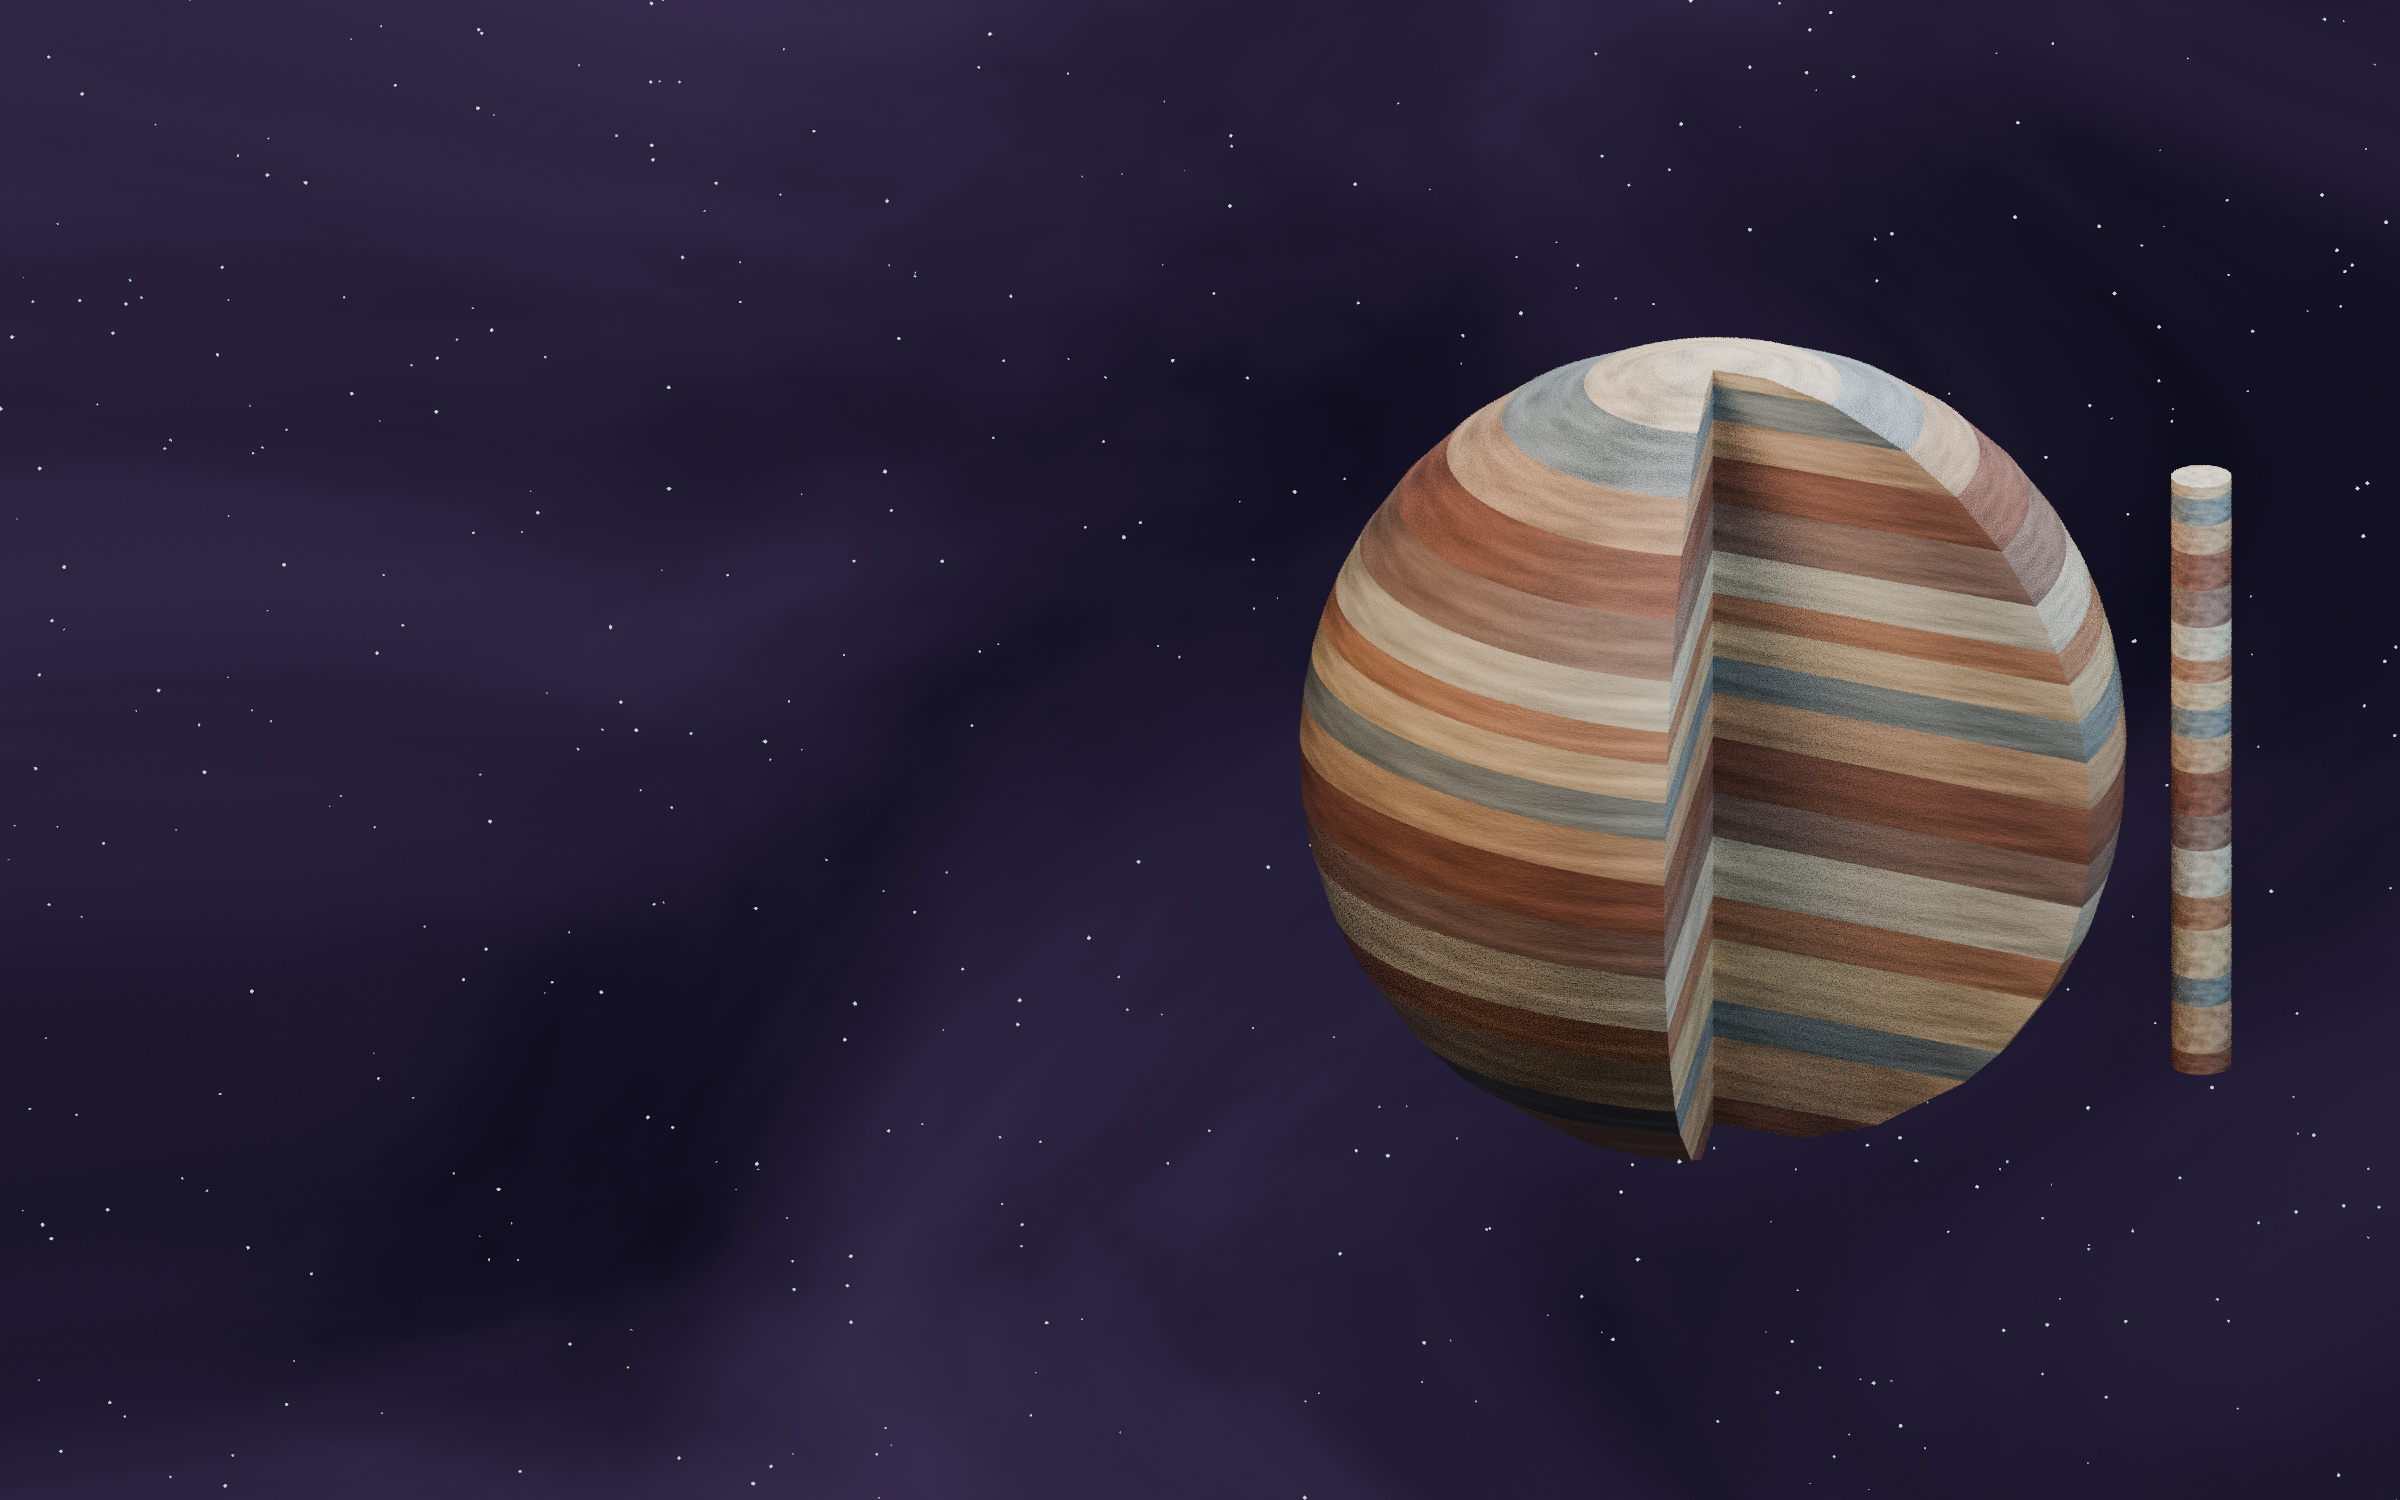
\includegraphics[width=20cm,height=12.5cm]{Scena/copertina.jpg}};}{}
\node[anchor=north west,inner sep=0] at([xshift=1.05cm,yshift=-1.10cm]current page.north west){\color{Mint}\bfseries\fontsize{23}{28}\selectfont STRATA};
\node[anchor=north west,inner sep=0] at([xshift=1.07cm,yshift=-2.16cm]current page.north west){\color{white}\fontsize{9}{12}\selectfont MODULO M13 · SCIENZE DELLA TERRA};
\draw[Mint,line width=1.5pt]([xshift=1.07cm,yshift=-2.78cm]current page.north west)--([xshift=2.6cm,yshift=-2.78cm]current page.north west);
\node[anchor=north west,inner sep=0] at([xshift=1.05cm,yshift=-3.35cm]current page.north west){\begin{minipage}{9.2cm}\raggedright\color{white}\bfseries\fontsize{28.5}{34.5}\selectfont Cronologie e archivi\\sedimentari\end{minipage}};
\node[anchor=north west,inner sep=0] at([xshift=1.07cm,yshift=-7.88cm]current page.north west){\begin{minipage}{8.9cm}\raggedright\color{Lilac}\fontsize{12.2}{17}\selectfont Il tempo registrato in una carota\end{minipage}};
\node[anchor=north west,inner sep=0] at([xshift=1.07cm,yshift=-8.70cm]current page.north west){\begin{minipage}{8.9cm}\raggedright\color{white!75}\fontsize{10.3}{14.5}\selectfont Ancore, proxy e incertezza cronologica\end{minipage}};
\node[anchor=north west,inner sep=0] at([xshift=1.07cm,yshift=-10.52cm]current page.north west){\color{white}\fontsize{10.5}{14}\selectfont GeoStat Lab · corso di Marzio De Corato};
\node[anchor=north west,inner sep=0] at([xshift=1.07cm,yshift=-11.17cm]current page.north west){\color{Mint}\fontsize{8.8}{11}\selectfont\href{https://creativecommons.org/licenses/by-nc-sa/4.0/}{Impaginazione da Tessera · CC BY-NC-SA 4.0}};
\end{tikzpicture}\end{frame}
\begin{frame}[plain]\hypertarget{slide2}{}
\bookmark[level=1,page=2]{Indice della presentazione}
\begin{tikzpicture}[remember picture,overlay]
\PilotChrome{Indice della presentazione}{PERCORSO}{2}{I titoli dell’indice aprono i capitoli. Il nome del capitolo in alto riporta a questa pagina.}
\node[anchor=north west,inner sep=0] at([xshift=.96cm,yshift=-2.12cm]current page.north west){\Colonna{9.40cm}{\PLabel{Capitoli}
{\fontsize{10.7}{13.5}\selectfont\hyperlink{slide4}{Archivio, ancore e convenzioni temporali\hfill 4}\par}\vspace{.16cm}
{\fontsize{10.7}{13.5}\selectfont\hyperlink{slide13}{Interpolazione e tassi di accumulo\hfill 13}\par}\vspace{.16cm}
{\fontsize{10.7}{13.5}\selectfont\hyperlink{slide22}{Scenari cronologici e propagazione\hfill 22}\par}\vspace{.16cm}
{\fontsize{10.7}{13.5}\selectfont\hyperlink{slide32}{Proxy e risoluzione temporale\hfill 32}\par}\vspace{.16cm}
{\fontsize{10.7}{13.5}\selectfont\hyperlink{slide41}{Discontinuità e sensibilità del modello\hfill 41}\par}\vspace{.16cm}
{\fontsize{10.7}{13.5}\selectfont\hyperlink{slide50}{Pendenze, durate ed eventi\hfill 50}\par}\vspace{.16cm}
{\fontsize{10.7}{13.5}\selectfont\hyperlink{slide59}{Consegna e studio autonomo\hfill 59}\par}\vspace{.16cm}
}};
\node[anchor=north west,inner sep=0] at([xshift=10.85cm,yshift=-2.12cm]current page.north west){\Colonna{8.16cm}{\PLabel{Percorso di lettura}
\PBody{La carota didattica è lunga 160 cm. Sei ancore sintetiche la collocano fra 0 e 2200 anni cal BP. Il proxy è misurato ogni 2 cm.}
\PInfo{Le pagine Scenario A e Confronto riprendono gli esperimenti nel browser. I valori di partenza del simulatore possono differire dal caso guida.}
\href{https://marzione00.github.io/Lab_Geo/\#modulo-M13}{\color{Classical}\bfseries Apri gli esperimenti di Strata}}};
\end{tikzpicture}\end{frame}

\begin{frame}[plain]\hypertarget{slide3}{}
\bookmark[level=1,page=3]{Quando si è depositato il livello in cui il proxy raggiunge il massimo osservato?}
\begin{tikzpicture}[remember picture,overlay]
\PilotChrome{{\fontsize{15.3}{19}\selectfont Quando si è depositato il livello in cui il proxy raggiunge il massimo osservato?}}{IL CASO GUIDA}{3}{Le ancore sono osservazioni del caso sintetico. Il tempo intermedio è una stima del modello.}
\node[anchor=north west,inner sep=0] at([xshift=.96cm,yshift=-2.12cm]current page.north west){\Colonna{9.40cm}{{\centering\resizebox{.97\linewidth}{!}{\begin{tikzpicture}[x=1cm,y=1cm]

\foreach \y/\col in {0/GeoA,0.62/GeoB,1.24/GeoC,1.86/GeoA,2.48/GeoB,3.10/GeoC,3.72/GeoB}{
 \fill[\col!37] (.5,\y) rectangle (1.8,{\y+.62});}
\draw[Navy] (.5,0) rectangle (1.8,4.34);
\node[pNote] at (1.15,4.72){carota};
\draw[pAxis] (3.15,4.3)--(7.85,4.3) node[above left,pNote]{età (cal BP)};
\draw[pAxis] (3.15,4.3)--(3.15,-.3) node[below,pNote]{cm};
\draw[GeoA,very thick] (3.15,4.3)--(3.48,3.76)--(4.09,2.96)--(4.78,2.15)--(6.08,1.08)--(7.75,0);
\foreach \dep/\xx/\yy in {0/3.15/4.3,20/3.48/3.76,50/4.09/2.96,80/4.78/2.15,120/6.08/1.08,160/7.75/0}{
 \draw[white,line width=.7pt] (.5,\yy)--(1.8,\yy);
 \draw[Muted!35,densely dotted] (1.8,\yy)--(\xx,\yy);
 \node[font=\scriptsize,fill=Paper,inner sep=1pt] at (2.48,\yy){\dep};
 \fill[GeoB] (\xx,\yy) circle(2.1pt);}
\node[pNote,anchor=north] at(6,3.55){sei ancore sintetiche};

\end{tikzpicture}
}\par}
}};
\node[anchor=north west,inner sep=0] at([xshift=10.85cm,yshift=-2.12cm]current page.north west){\Colonna{8.16cm}{\PLabel{Il caso}
\PBody{La carota didattica è lunga 160 cm. Sei ancore sintetiche la collocano fra 0 e 2200 anni cal BP. Il proxy è misurato ogni 2 cm.}
\PInfo{Costruiremo una curva età–profondità, ne controlleremo il dominio e confronteremo la datazione del massimo con uno scenario che contiene una lacuna.}
}};
\end{tikzpicture}\end{frame}

\begin{frame}[plain]\hypertarget{slide4}{}
\bookmark[level=0,page=4]{Archivio, ancore e convenzioni temporali}
\bookmark[level=1,page=4]{Quanto tempo separa due livelli della carota?}
\begin{tikzpicture}[remember picture,overlay]
\PilotChrome{Quanto tempo separa due livelli della carota?}{ARCHIVIO, ANCORE E CONVENZIONI TEMPORALI}{4}{Conserva unite coordinate di profondità ed età di ogni ancora.}
\node[anchor=north west,inner sep=0] at([xshift=.96cm,yshift=-2.12cm]current page.north west){\Colonna{9.40cm}{\PLabel{Domanda}
\PBody{Una carota sintetica attraversa 160 cm di sedimento e contiene sei livelli datati. Prima di interpolare chiediamoci dove sono davvero collocati i vincoli.}
\vspace{.35cm}\PLabel{Interpretazione}
\PBody{Tra 20 e 50 cm passano 290 anni. Lo stesso spessore può registrare una durata diversa in un altro segmento.}
}};
\node[anchor=north west,inner sep=0] at([xshift=10.85cm,yshift=-2.12cm]current page.north west){\Colonna{8.16cm}{\begin{tcolorbox}[enhanced,arc=1.7mm,boxrule=.6pt,colback=white,colframe=Classical!60!Navy,colbacktitle=Navy,coltitle=white,fonttitle=\bfseries\small,title={R · calcolo riproducibile},left=1.7mm,right=1.3mm,top=1.1mm,bottom=1.1mm,before skip=1mm,after skip=1.0mm]\lstinputlisting[style=GeoR,language=R]{Codice/capitolo-01.R}\end{tcolorbox}
\PLabel{Risultato in R}
\begin{tcolorbox}[colback=GeoTint,colframe=Rule,boxrule=.5pt,arc=1.4mm,left=2mm,right=1mm,top=1mm,bottom=1mm]{\fontsize{9}{12}\selectfont\ttfamily \mbox{cm\ anni\ }\\\mbox{\ \ 30\ \ 290}}\end{tcolorbox}}};
\end{tikzpicture}\end{frame}

\begin{frame}[plain]\hypertarget{slide5}{}
\bookmark[level=1,page=5]{La cronologia collega profondità e tempo}
\begin{tikzpicture}[remember picture,overlay]
\PilotChrome{La cronologia collega profondità e tempo}{ARCHIVIO, ANCORE E CONVENZIONI TEMPORALI}{5}{Il passaggio dalla profondità al tempo richiede un modello cronologico esplicito.}
\node[anchor=north west,inner sep=0] at([xshift=.96cm,yshift=-2.12cm]current page.north west){\Colonna{9.40cm}{{\centering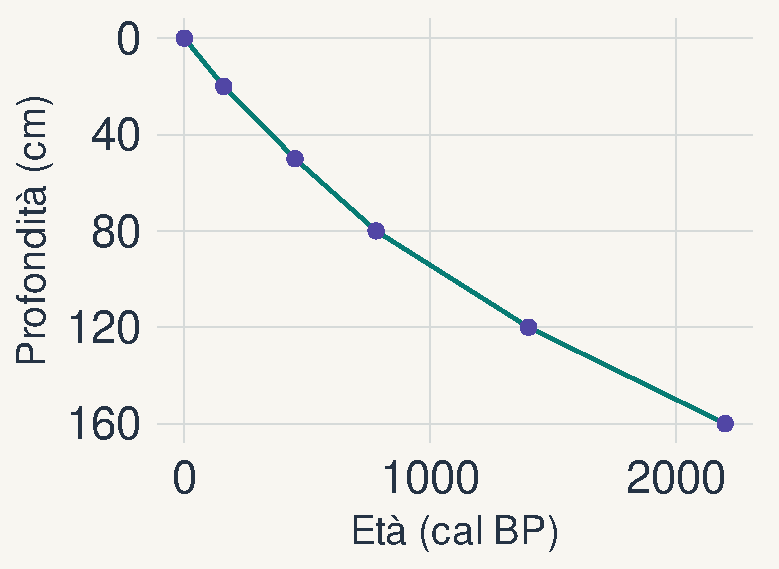
\includegraphics[width=\linewidth,height=6.15cm,keepaspectratio]{Figure/F01.pdf}\par}
\PSmall{Sei ancore sintetiche e interpolazione lineare a tratti. La profondità aumenta verso il basso.}
}};
\node[anchor=north west,inner sep=0] at([xshift=10.85cm,yshift=-2.12cm]current page.north west){\Colonna{8.16cm}{\PBody{Un archivio sedimentario conserva osservazioni ordinate nello spazio stratigrafico, mentre l’interpretazione temporale richiede una relazione fra profondità ed età. Il capitolo utilizza sei ancore sintetiche distribuite fra zero e 160 centimetri, con età di calendario comprese fra zero e 2200 anni BP. Un proxy simulato è disponibile ogni due centimetri. Le deviazioni standard associate alle ancore definiscono scenari didattici di sensibilità, dei quali occorre conservare la natura ipotetica quando si interpretano bande e durate derivate.}
\par\smallskip{\centering\adjustbox{max width=.98\linewidth}{$\displaystyle t=t(z),\qquad z\in[0,160]\ \mathrm{cm}$}\par\smallskip}
}};
\end{tikzpicture}\end{frame}

\begin{frame}[plain]\hypertarget{slide6}{}
\bookmark[level=1,page=6]{L’associazione fra ancora ed evidenza stratigrafica}
\begin{tikzpicture}[remember picture,overlay]
\PilotChrome{L’associazione fra ancora ed evidenza stratigrafica}{ARCHIVIO, ANCORE E CONVENZIONI TEMPORALI}{6}{La coppia età–profondità costituisce l’unità informativa che il controllo deve preservare.}
\node[anchor=north west,inner sep=0] at([xshift=.96cm,yshift=-2.12cm]current page.north west){\Colonna{9.40cm}{{\centering\resizebox{.97\linewidth}{!}{\begin{tikzpicture}[x=1cm,y=-.87cm,every node/.style={font=\fontsize{12.2}{15}\selectfont,text=Ink},arr/.style={-{Stealth[length=2mm]},line width=.8pt,draw=Classical}]\path[use as bounding box] (0,0) rectangle (7.45,6.2);
\draw[draw=Classical,fill=Classical!8,rounded corners=2pt,line width=.7pt] (0.8,0.7) rectangle (2.3,5.6);
\draw[Quantum,line width=.8pt] (0.8,0.9)--(2.3,0.9);
\node[anchor=center,text=Ink,font=\fontsize{11}{15}\selectfont,text width=4cm,align=center] at (4.6,0.9) {0 cm · 0 cal BP};
\draw[Quantum,line width=.8pt] (0.8,1.475)--(2.3,1.475);
\node[anchor=center,text=Ink,font=\fontsize{11}{15}\selectfont,text width=4cm,align=center] at (4.6,1.475) {20 cm · 160 cal BP};
\draw[Quantum,line width=.8pt] (0.8,2.3375)--(2.3,2.3375);
\node[anchor=center,text=Ink,font=\fontsize{11}{15}\selectfont,text width=4cm,align=center] at (4.6,2.3375) {50 cm · 450 cal BP};
\draw[Quantum,line width=.8pt] (0.8,3.2)--(2.3,3.2);
\node[anchor=center,text=Ink,font=\fontsize{11}{15}\selectfont,text width=4cm,align=center] at (4.6,3.2) {80 cm · 780 cal BP};
\draw[Quantum,line width=.8pt] (0.8,4.3500000000000005)--(2.3,4.3500000000000005);
\node[anchor=center,text=Ink,font=\fontsize{11}{15}\selectfont,text width=4cm,align=center] at (4.6,4.3500000000000005) {120 cm · 1400 cal BP};
\draw[Quantum,line width=.8pt] (0.8,5.500000000000001)--(2.3,5.500000000000001);
\node[anchor=center,text=Ink,font=\fontsize{11}{15}\selectfont,text width=4cm,align=center] at (4.6,5.500000000000001) {160 cm · 2200 cal BP};

\end{tikzpicture}}\par}
}};
\node[anchor=north west,inner sep=0] at([xshift=10.85cm,yshift=-2.12cm]current page.north west){\Colonna{8.16cm}{\PBody{Ogni ancora lega un’età a una profondità e a un insieme di metadati, che nelle indagini reali comprende materiale, metodo, identificativo e contesto deposizionale. Il controllo ordina le righe per profondità e verifica la coerenza delle età, mantenendo intatte le coppie. Ordinare separatamente le età altererebbe l’associazione con i livelli, cancellando l’evidenza di eventuali inversioni. La monotonicità può essere un’ipotesi geologica pertinente per una successione indisturbata, la cui validità deve essere valutata prima di imporla al modello.}
\par\smallskip{\centering\adjustbox{max width=.98\linewidth}{$\displaystyle z_{i+1}>z_i,\qquad t_{i+1}>t_i\quad\text{nel modello monotono}$}\par\smallskip}
}};
\end{tikzpicture}\end{frame}

\begin{frame}[plain]\hypertarget{slide7}{}
\bookmark[level=1,page=7]{Origine BP e rappresentazione dell’anno civile}
\begin{tikzpicture}[remember picture,overlay]
\PilotChrome{Origine BP e rappresentazione dell’anno civile}{ARCHIVIO, ANCORE E CONVENZIONI TEMPORALI}{7}{L’origine convenzionale e la notazione dell’anno devono accompagnare ogni cronologia.}
\node[anchor=north west,inner sep=0] at([xshift=.96cm,yshift=-2.12cm]current page.north west){\Colonna{9.40cm}{{\centering\resizebox{.97\linewidth}{!}{\begin{tikzpicture}[x=1cm,y=-.87cm,every node/.style={font=\fontsize{12.2}{15}\selectfont,text=Ink},arr/.style={-{Stealth[length=2mm]},line width=.8pt,draw=Classical}]\path[use as bounding box] (0,0) rectangle (7.45,6.2);
\draw[arr,draw=Classical] (0.5,3)--(7,3);
\draw[Quantum,line width=.8pt] (1,2.5)--(1,3.5);
\draw[Classical,line width=.8pt] (3.4,2.5)--(3.4,3.5);
\draw[Classical,line width=.8pt] (6.1,2.5)--(6.1,3.5);
\node[anchor=center,text=Ink,font=\fontsize{11}{15}\selectfont] at (1,1.8) {1 a.C.};
\node[anchor=center,text=Ink,font=\fontsize{11}{15}\selectfont] at (3.4,1.8) {1 d.C.};
\node[anchor=center,text=Ink,font=\fontsize{11}{15}\selectfont] at (6.1,1.8) {1950 d.C.};
\node[anchor=center,text=Ink,font=\fontsize{11}{15}\selectfont] at (1,4.2) {Anno 0};
\node[anchor=center,text=Ink,font=\fontsize{11}{15}\selectfont] at (3.4,4.2) {Anno 1};
\node[anchor=center,text=Ink,font=\fontsize{11}{15}\selectfont] at (6.1,4.2) {0 cal BP};
\node[anchor=center,text=Ink,font=\fontsize{11}{15}\selectfont,text width=6.8cm,align=center] at (3.7,5.5) {Schema delle convenzioni, senza scala uniforme.};

\end{tikzpicture}}\par}
}};
\node[anchor=north west,inner sep=0] at([xshift=10.85cm,yshift=-2.12cm]current page.north west){\Colonna{8.16cm}{\PBody{La convenzione BP fissa il presente al 1950, indipendentemente dall’anno nel quale si esegue l’analisi. Per età già espresse in anni di calendario BP, la sottrazione da 1950 produce una coordinata sulla scala degli anni astronomici. Il passaggio alle etichette a.C. e d.C. richiede attenzione all’assenza dell’anno zero nella notazione storica: l’anno astronomico zero corrisponde al primo anno avanti Cristo. Le età negative in cal BP individuerebbero invece tempi successivi al riferimento convenzionale.}
\par\smallskip{\centering\adjustbox{max width=.98\linewidth}{$\displaystyle y_{\rm astronomico}=1950-t_{\rm cal\ BP}$}\par\smallskip}
}};
\end{tikzpicture}\end{frame}

\begin{frame}[plain]\hypertarget{slide8}{}
\bookmark[level=1,page=8]{Età radiocarbonica e calibrazione}
\begin{tikzpicture}[remember picture,overlay]
\PilotChrome{Età radiocarbonica e calibrazione}{ARCHIVIO, ANCORE E CONVENZIONI TEMPORALI}{8}{Calibrazione della datazione e interpolazione età–profondità sono operazioni scientifiche distinte.}
\node[anchor=north west,inner sep=0] at([xshift=.96cm,yshift=-2.12cm]current page.north west){\Colonna{9.40cm}{\PLabel{Metodo}
\PBody{Un’età radiocarbonica convenzionale richiede una calibrazione per essere espressa sulla scala del calendario, poiché la relazione fra le due scale dipende dalla storia del radiocarbonio e dal contesto del campione. Una semplice sottrazione da 1950 non esegue tale operazione. Curve di calibrazione, ambiente di formazione ed eventuali effetti di riserva devono essere scelti in modo pertinente. Le sei ancore del laboratorio sono già età di calendario inventate, per cui l’esercizio affronta la costruzione della cronologia senza simulare una calibrazione radiocarbonica reale.}
}};
\node[anchor=north west,inner sep=0] at([xshift=10.85cm,yshift=-2.12cm]current page.north west){\Colonna{8.16cm}{\PLabel{Interpretazione}
\PBody{Una distribuzione calibrata può essere asimmetrica o multimodale. Riassumerla automaticamente mediante una media e una deviazione standard può perdere informazione utile alla costruzione del modello stratigrafico. I dati reali richiedono la conservazione del risultato di calibrazione e delle sue assunzioni.}
}};
\end{tikzpicture}\end{frame}

\begin{frame}[plain]\hypertarget{slide9}{}
\bookmark[level=1,page=9]{Sei ancore delimitano il dominio}
\begin{tikzpicture}[remember picture,overlay]
\PilotChrome{Sei ancore delimitano il dominio}{ARCHIVIO, ANCORE E CONVENZIONI TEMPORALI}{9}{Le sei ancore si distribuiscono fra la superficie e 160 cm.}
\node[anchor=north west,inner sep=0] at([xshift=.96cm,yshift=-2.12cm]current page.north west){\Colonna{9.40cm}{\PLabel{Risultati del caso R6}
{\fontsize{10.2}{12.8}\selectfont\begin{tabular}{@{}>{\raggedright\arraybackslash}p{0.52\linewidth}@{\hspace{.13cm}}>{\raggedright\arraybackslash}p{0.39\linewidth}@{}}\toprule Grandezza & Valore\\[2.3pt]
\midrule 
Numero & 6\\[2.3pt]
Min. cm & 0\\[2.3pt]
Max cm & 160\\[2.3pt]
Età max BP & 2200\\[2.3pt]
\bottomrule\end{tabular}\par}
}};
\node[anchor=north west,inner sep=0] at([xshift=10.85cm,yshift=-2.12cm]current page.north west){\Colonna{8.16cm}{\PBody{Quale parte della carota è effettivamente vincolata da una datazione?}
\vspace{.4cm}\PInfo{Le sei ancore si distribuiscono fra la superficie e 160 cm. Gli estremi delimitano l’intervallo di interpolazione, mentre la distanza fra le ancore ne descrive il sostegno locale.}
}};
\node[anchor=north east,inner sep=0] at([xshift=17.1cm,yshift=-12.04cm]current page.north west){\fontsize{7.7}{9}\selectfont \href{https://github.com/marzione00/Lab_Geo/blob/649f7cc577b96bd1044d81e78a2f530813e4f96b/materiali/laboratori/M13/M13_N01.R}{\color{Classical}\bfseries Script R · M13\_N01}};
\end{tikzpicture}\end{frame}

\begin{frame}[plain]\hypertarget{slide10}{}
\bookmark[level=1,page=10]{Gli intervalli fra ancore hanno ampiezze diverse}
\begin{tikzpicture}[remember picture,overlay]
\PilotChrome{Gli intervalli fra ancore hanno ampiezze diverse}{ARCHIVIO, ANCORE E CONVENZIONI TEMPORALI}{10}{Confronta le differenze in anni e centimetri.}
\node[anchor=north west,inner sep=0] at([xshift=.96cm,yshift=-2.12cm]current page.north west){\Colonna{9.40cm}{\PLabel{Risultati del caso R6}
{\fontsize{10.2}{12.8}\selectfont\begin{tabular}{@{}>{\raggedright\arraybackslash}p{0.22\linewidth}@{\hspace{.13cm}}>{\raggedright\arraybackslash}p{0.22\linewidth}@{\hspace{.13cm}}>{\raggedright\arraybackslash}p{0.22\linewidth}@{\hspace{.13cm}}>{\raggedright\arraybackslash}p{0.23\linewidth}@{}}\toprule Da (cm) & A (cm) & $\Delta$ cm & $\Delta$ anni\\[2.3pt]
\midrule 
0 & 20 & 20 & 160\\[2.3pt]
20 & 50 & 30 & 290\\[2.3pt]
50 & 80 & 30 & 330\\[2.3pt]
80 & 120 & 40 & 620\\[2.3pt]
120 & 160 & 40 & 800\\[2.3pt]
\bottomrule\end{tabular}\par}
}};
\node[anchor=north west,inner sep=0] at([xshift=10.85cm,yshift=-2.12cm]current page.north west){\Colonna{8.16cm}{\PBody{Dove si accumula più tempo fra due misure cronologiche consecutive?}
\vspace{.4cm}\PInfo{Confronta le differenze in anni e centimetri. Il primo segmento attraversa 20 cm in 160 anni, l’ultimo 40 cm in 800 anni.}
}};
\node[anchor=north east,inner sep=0] at([xshift=17.1cm,yshift=-12.04cm]current page.north west){\fontsize{7.7}{9}\selectfont \href{https://github.com/marzione00/Lab_Geo/blob/649f7cc577b96bd1044d81e78a2f530813e4f96b/materiali/laboratori/M13/M13_N03.R}{\color{Classical}\bfseries Script R · M13\_N03}};
\end{tikzpicture}\end{frame}

\begin{frame}[plain]\hypertarget{slide11}{}
\bookmark[level=1,page=11]{Ancore cronologiche e convenzioni temporali}
\begin{tikzpicture}[remember picture,overlay]
\PilotChrome{Ancore cronologiche e convenzioni temporali}{ARCHIVIO, ANCORE E CONVENZIONI TEMPORALI}{11}{Collegare profondità, età e riferimento temporale.}
\node[anchor=north west,inner sep=0] at([xshift=.96cm,yshift=-2.12cm]current page.north west){\Colonna{9.40cm}{{\centering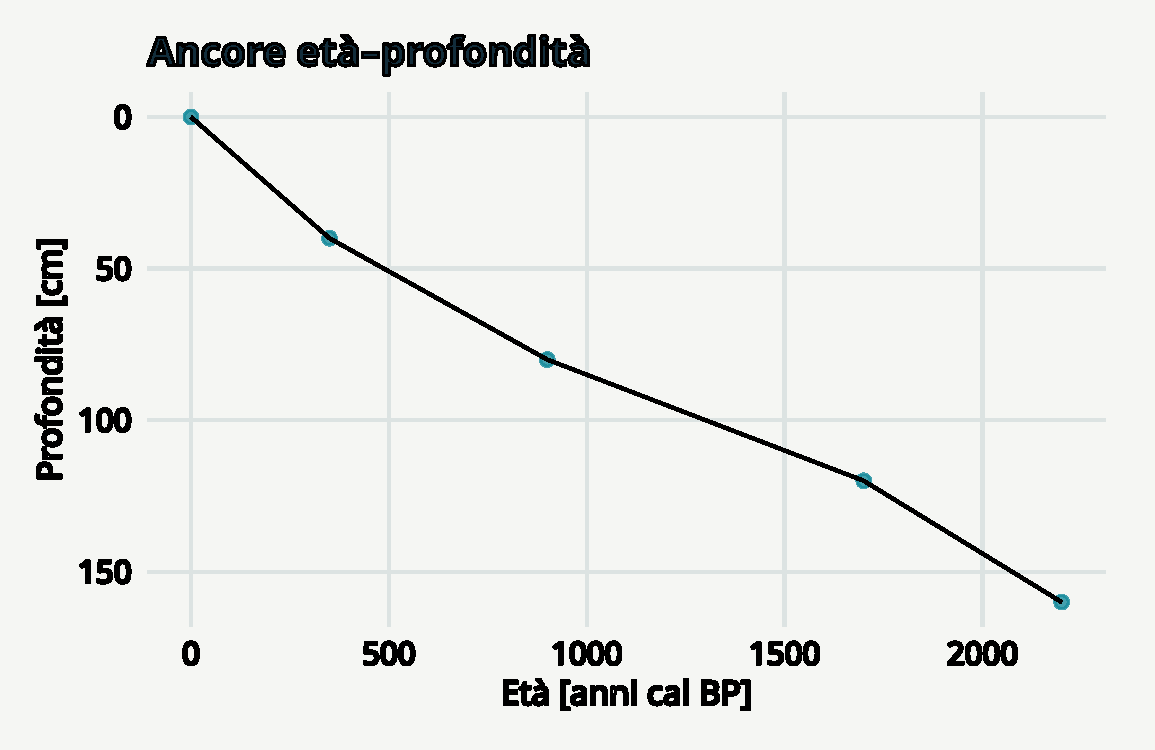
\includegraphics[width=\linewidth,height=6.0cm,keepaspectratio]{Esperimenti/m13-ancore-A.pdf}\par}
\PSmall{Età dell’ancora a 80 cm [anni cal BP]: 900. Seme: 17.}
}};
\node[anchor=north west,inner sep=0] at([xshift=10.85cm,yshift=-2.12cm]current page.north west){\Colonna{8.16cm}{\PLabel{Scenario A · simulazione}
\PBody{Un’ancora cronologica associa una profondità a un’età, mantenendo il legame con il livello stratigrafico dal quale deriva. Le cinque ancore dell’esperimento sono sintetiche e già espresse in anni di calendario BP; il controllo modifica quella situata a ottanta centimetri. La carta mostra come questa scelta cambi la relazione locale fra spessore ed età.}
\par\smallskip{\centering\adjustbox{max width=.98\linewidth}{$\displaystyle a_{astronomico}=1950-t_{cal\,BP}$}\par\smallskip}
\PSmall{$T_{\mathrm{cal\,BP}}$ è l’età di calendario rispetto al 1950; l’anno astronomico si ottiene sottraendo tale età da 1950. Profondità crescenti ed età crescenti definiscono la monotonicità controllata dal programma.}
}};
\node[anchor=north east,inner sep=0] at([xshift=17.1cm,yshift=-12.04cm]current page.north west){\fontsize{7.7}{9}\selectfont \href{https://marzione00.github.io/Lab_Geo/\#laboratorio/m13-ancore}{\color{Classical}\bfseries Apri il laboratorio · m13-ancore}};
\end{tikzpicture}\end{frame}

\begin{frame}[plain]\hypertarget{slide12}{}
\bookmark[level=1,page=12]{Confronto | Ancore cronologiche e convenzioni temporali}
\begin{tikzpicture}[remember picture,overlay]
\PilotChrome{Confronto | Ancore cronologiche e convenzioni temporali}{ARCHIVIO, ANCORE E CONVENZIONI TEMPORALI}{12}{Le ancore associano età e profondità; la convenzione BP usa il 1950 come riferimento.}
\node[anchor=north west,inner sep=0] at([xshift=.96cm,yshift=-2.12cm]current page.north west){\Colonna{9.40cm}{{\centering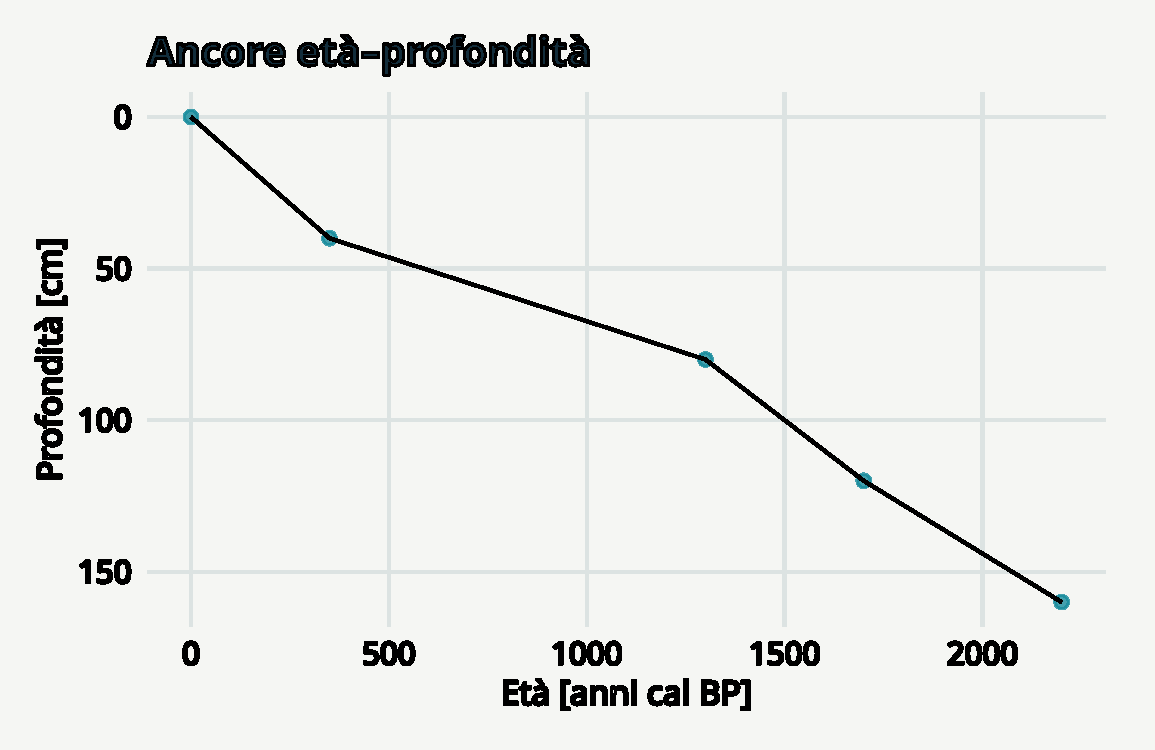
\includegraphics[width=\linewidth,height=5.6cm,keepaspectratio]{Esperimenti/m13-ancore-B.pdf}\par}
\PSmall{Età dell’ancora a 80 cm [anni cal BP]: 900 $\to$ 1300. Tutti gli altri parametri e il seme sono fissi.}
}};
\node[anchor=north west,inner sep=0] at([xshift=10.85cm,yshift=-2.12cm]current page.north west){\Colonna{8.16cm}{\PLabel{Confronto fra gli scenari}
{\fontsize{10.2}{12.8}\selectfont\begin{tabular}{@{}>{\raggedright\arraybackslash}p{0.48\linewidth}@{\hspace{.13cm}}>{\raggedright\arraybackslash}p{0.224\linewidth}@{\hspace{.13cm}}>{\raggedright\arraybackslash}p{0.224\linewidth}@{}}\toprule Grandezza & A & B\\[2.3pt]
\midrule 
Anno astronomico dell’ancora & 1050 & 650\\[2.3pt]
Ancore & 5 & 5\\[2.3pt]
Cronologia monotona & 1 & 1\\[2.3pt]
\bottomrule\end{tabular}\par}
\vspace{.25cm}\PBody{Portando l’ancora da 900 a 1300 anni BP, l’anno astronomico corrispondente passa da 1050 a 650. Le cinque ancore del simulatore conservano l’ordine.}
}};
\node[anchor=north east,inner sep=0] at([xshift=17.1cm,yshift=-12.04cm]current page.north west){\fontsize{7.7}{9}\selectfont \href{https://marzione00.github.io/Lab_Geo/\#laboratorio/m13-ancore}{\color{Classical}\bfseries Apri il laboratorio · m13-ancore}};
\end{tikzpicture}\end{frame}

\begin{frame}[plain]\hypertarget{slide13}{}
\bookmark[level=0,page=13]{Interpolazione e tassi di accumulo}
\bookmark[level=1,page=13]{Un livello a 35 cm cade fra due ancore}
\begin{tikzpicture}[remember picture,overlay]
\PilotChrome{Un livello a 35 cm cade fra due ancore}{INTERPOLAZIONE E TASSI DI ACCUMULO}{13}{La retta tra ancore formalizza una scelta sul processo di accumulo.}
\node[anchor=north west,inner sep=0] at([xshift=.96cm,yshift=-2.12cm]current page.north west){\Colonna{9.40cm}{\PLabel{Domanda}
\PBody{Fra 20 cm e 50 cm, l’età passa da 160 a 450 anni cal BP. Dove collocheresti temporalmente il livello a 35 cm?}
\vspace{.35cm}\PLabel{Interpretazione}
\PBody{Il livello è a metà del segmento. Con accumulo costante l’età è a metà fra le datazioni, ossia 305 anni cal BP.}
}};
\node[anchor=north west,inner sep=0] at([xshift=10.85cm,yshift=-2.12cm]current page.north west){\Colonna{8.16cm}{\begin{tcolorbox}[enhanced,arc=1.7mm,boxrule=.6pt,colback=white,colframe=Classical!60!Navy,colbacktitle=Navy,coltitle=white,fonttitle=\bfseries\small,title={R · calcolo riproducibile},left=1.7mm,right=1.3mm,top=1.1mm,bottom=1.1mm,before skip=1mm,after skip=1.0mm]\lstinputlisting[style=GeoR,language=R]{Codice/capitolo-02.R}\end{tcolorbox}
\PLabel{Risultato in R}
\begin{tcolorbox}[colback=GeoTint,colframe=Rule,boxrule=.5pt,arc=1.4mm,left=2mm,right=1mm,top=1mm,bottom=1mm]{\fontsize{9}{12}\selectfont\ttfamily \mbox{[1]\ 305}}\end{tcolorbox}}};
\end{tikzpicture}\end{frame}

\begin{frame}[plain]\hypertarget{slide14}{}
\bookmark[level=1,page=14]{Interpolazione lineare fra due ancore}
\begin{tikzpicture}[remember picture,overlay]
\PilotChrome{Interpolazione lineare fra due ancore}{INTERPOLAZIONE E TASSI DI ACCUMULO}{14}{L’interpolazione incorpora un’ipotesi sul comportamento fra le ancore.}
\node[anchor=north west,inner sep=0] at([xshift=.96cm,yshift=-2.12cm]current page.north west){\Colonna{9.40cm}{{\centering\resizebox{.97\linewidth}{!}{\begin{tikzpicture}[x=1cm,y=-.87cm,every node/.style={font=\fontsize{12.2}{15}\selectfont,text=Ink},arr/.style={-{Stealth[length=2mm]},line width=.8pt,draw=Classical}]\path[use as bounding box] (0,0) rectangle (7.45,6.2);
\draw[arr,draw=Classical] (0.6,3)--(6.9,3);
\draw[Quantum,line width=.8pt] (1,2.6)--(1,3.4);
\draw[Quantum,line width=.8pt] (3.7,2.6)--(3.7,3.4);
\draw[Quantum,line width=.8pt] (6.4,2.6)--(6.4,3.4);
\node[anchor=center,text=Ink,font=\fontsize{11}{15}\selectfont,text width=1.8cm,align=center] at (1,1.8) {20 cm\par160 anni};
\node[anchor=center,text=Ink,font=\fontsize{11}{15}\selectfont,text width=2cm,align=center] at (3.7,1.8) {35 cm\par305 anni};
\node[anchor=center,text=Ink,font=\fontsize{11}{15}\selectfont,text width=1.8cm,align=center] at (6.4,1.8) {50 cm\par450 anni};
\node[anchor=center,text=Ink,font=\fontsize{16}{15}\selectfont] at (3.7,4.5) {λ = 1/2};
\node[anchor=center,text=Ink,font=\fontsize{11}{15}\selectfont,text width=6.8cm,align=center] at (3.7,5.6) {La posizione intermedia assegna pesi uguali.};

\end{tikzpicture}}\par}
\PSmall{$z_i,t_i$: profondità ed età dell’ancora i; $\lambda$: peso dell’ancora successiva. Esempio in cm e anni cal BP, riferiti al 1950.}
}};
\node[anchor=north west,inner sep=0] at([xshift=10.85cm,yshift=-2.12cm]current page.north west){\Colonna{8.16cm}{\PBody{Fra due profondità adiacenti, l’interpolazione lineare combina le rispettive età con pesi determinati dalla posizione relativa. Il modello assume che il tasso apparente resti costante entro quel segmento e consente che cambi attraversando un’ancora. A 35 centimetri, posizione intermedia fra 20 e 50 centimetri, i pesi sono entrambi un mezzo e l’età risulta pari a 305 anni cal BP. Il passaggio esatto per le ancore deriva dalla definizione dell’interpolatore e non costituisce una verifica indipendente della cronologia.}
\par\smallskip{\centering\adjustbox{max width=.98\linewidth}{$\displaystyle \lambda=\frac{z-z_i}{z_{i+1}-z_i},\qquad t(z)=(1-\lambda)t_i+\lambda t_{i+1}$}\par\smallskip}
}};
\end{tikzpicture}\end{frame}

\begin{frame}[plain]\hypertarget{slide15}{}
\bookmark[level=1,page=15]{Il dominio dell’interpolazione in R}
\begin{tikzpicture}[remember picture,overlay]
\PilotChrome{Il dominio dell’interpolazione in R}{INTERPOLAZIONE E TASSI DI ACCUMULO}{15}{Ogni estrapolazione introduce ipotesi ulteriori rispetto all’interpolazione nel dominio osservato.}
\node[anchor=north west,inner sep=0] at([xshift=.96cm,yshift=-2.12cm]current page.north west){\Colonna{9.40cm}{\begin{tcolorbox}[enhanced,arc=1.7mm,boxrule=.6pt,colback=white,colframe=Classical!60!Navy,colbacktitle=Navy,coltitle=white,fonttitle=\bfseries\small,title={R · procedura},left=1.7mm,right=1.3mm,top=1.1mm,bottom=1.1mm,before skip=1mm,after skip=1.0mm]\lstinputlisting[style=GeoR,language=R]{Codice/lettura-08.R}\end{tcolorbox}
}};
\node[anchor=north west,inner sep=0] at([xshift=10.85cm,yshift=-2.12cm]current page.north west){\Colonna{8.16cm}{\PBody{La funzione approx restituisce valori entro il dominio delimitato dalle ancore, mentre rule uguale a uno rende esplicita la mancanza di una previsione esterna. Stimare l’età a 180 centimetri richiederebbe un’ipotesi aggiuntiva sul tasso oltre l’ultima ancora. Prolungare l’ultimo segmento oppure mantenere costante l’età estrema definisce due modelli differenti, che devono essere motivati separatamente. Il controllo manuale a 35 centimetri e la verifica dei valori esterni costituiscono prove semplici della coerenza dell’implementazione.}
}};
\end{tikzpicture}\end{frame}

\begin{frame}[plain]\hypertarget{slide16}{}
\bookmark[level=1,page=16]{Tasso apparente di accumulo e rapporto inverso}
\begin{tikzpicture}[remember picture,overlay]
\PilotChrome{Tasso apparente di accumulo e rapporto inverso}{INTERPOLAZIONE E TASSI DI ACCUMULO}{16}{Il tasso deve essere accompagnato dall’unità e dalle condizioni stratigrafiche della sua interpretazione.}
\node[anchor=north west,inner sep=0] at([xshift=.96cm,yshift=-2.12cm]current page.north west){\Colonna{9.40cm}{{\centering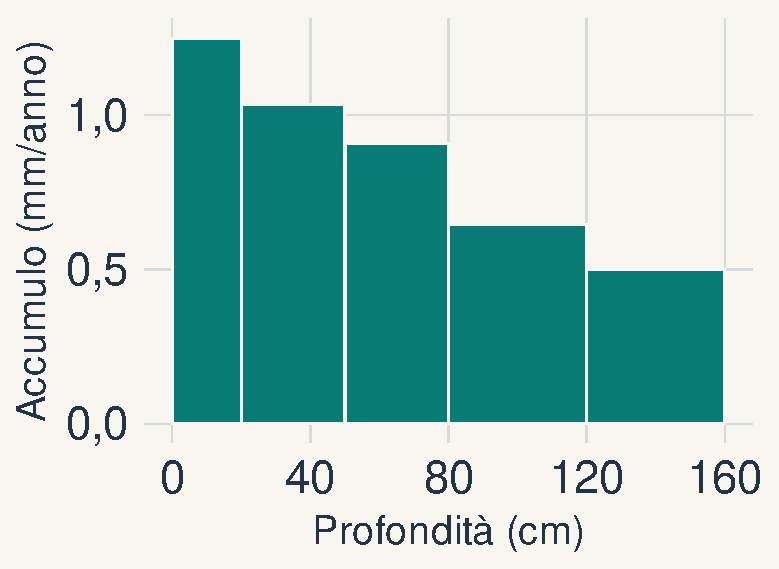
\includegraphics[width=\linewidth,height=6.15cm,keepaspectratio]{Figure/F02.pdf}\par}
\PSmall{z in cm, t in anni: $r_i$ è in cm/anno. L’asse mostra $10r_i$ in mm/anno; le barre seguono gli intervalli di profondità.}
}};
\node[anchor=north west,inner sep=0] at([xshift=10.85cm,yshift=-2.12cm]current page.north west){\Colonna{8.16cm}{\PBody{Il rapporto fra incremento di profondità e intervallo temporale esprime un tasso apparente di accumulo, mentre il suo inverso misura anni per centimetro. Il termine apparente ricorda che spessore attuale, compattazione, erosione e lacune possono rendere il rapporto diverso da un flusso deposizionale originario. Nella successione sintetica tutti i segmenti hanno incrementi positivi. La conversione da centimetri per anno a millimetri per anno moltiplica per dieci e deve essere applicata ai valori prima di modificarne l’etichetta.}
\par\smallskip{\centering\adjustbox{max width=.98\linewidth}{$\displaystyle r_i=\frac{z_{i+1}-z_i}{t_{i+1}-t_i},\qquad\frac{\mathrm dt}{\mathrm dz}=\frac1{r_i}$}\par\smallskip}
}};
\end{tikzpicture}\end{frame}

\begin{frame}[plain]\hypertarget{slide17}{}
\bookmark[level=1,page=17]{Media dei tassi e ponderazione temporale}
\begin{tikzpicture}[remember picture,overlay]
\PilotChrome{Media dei tassi e ponderazione temporale}{INTERPOLAZIONE E TASSI DI ACCUMULO}{17}{La ponderazione deriva dalla domanda alla quale deve rispondere il tasso medio.}
\node[anchor=north west,inner sep=0] at([xshift=.96cm,yshift=-2.12cm]current page.north west){\Colonna{9.40cm}{{\centering\resizebox{.97\linewidth}{!}{\begin{tikzpicture}[x=1cm,y=-.87cm,every node/.style={font=\fontsize{12.2}{15}\selectfont,text=Ink},arr/.style={-{Stealth[length=2mm]},line width=.8pt,draw=Classical}]\path[use as bounding box] (0,0) rectangle (7.45,6.2);
\draw[draw=Classical,fill=Classical!8,rounded corners=2pt,line width=.7pt] (0.6,1.2) rectangle (2.1,3.7);
\draw[draw=Quantum,fill=Quantum!8,rounded corners=2pt,line width=.7pt] (2.3,1.2) rectangle (6.8,3.7);
\node[anchor=center,text=Ink,font=\fontsize{16}{15}\selectfont] at (1.35,2.45) {$\Delta t_1$};
\node[anchor=center,text=Ink,font=\fontsize{16}{15}\selectfont] at (4.55,2.45) {$\Delta t_2$};
\node[anchor=center,text=Ink,font=\fontsize{12.2}{15}\selectfont,text width=6.8cm,align=center] at (3.7,4.6) {Il tempo trascorso determina il peso.};
\node[anchor=center,text=Ink,font=\fontsize{11}{15}\selectfont,text width=6.8cm,align=center] at (3.7,5.6) {Uno spessore totale, una durata totale.};

\end{tikzpicture}}\par}
}};
\node[anchor=north west,inner sep=0] at([xshift=10.85cm,yshift=-2.12cm]current page.north west){\Colonna{8.16cm}{\PBody{La media semplice dei cinque tassi assegna uguale peso a ogni segmento, benché i segmenti abbiano durate differenti. Per descrivere l’accumulo medio lungo l’intero periodo si ponderano invece i tassi per le rispettive durate; il risultato coincide con il rapporto fra spessore totale e durata complessiva. Nel caso didattico, 160 centimetri in 2200 anni corrispondono a circa 0,727 millimetri per anno. Il confronto rende esplicita la popolazione implicita nella media: segmenti equiponderati oppure tempo trascorso.}
\par\smallskip{\centering\adjustbox{max width=.98\linewidth}{$\displaystyle \overline r_{\Delta t}=\frac{\sum_i\Delta t_i r_i}{\sum_i\Delta t_i}=\frac{\sum_i\Delta z_i}{\sum_i\Delta t_i}$}\par\smallskip}
}};
\end{tikzpicture}\end{frame}

\begin{frame}[plain]\hypertarget{slide18}{}
\bookmark[level=1,page=18]{Due richieste cadono oltre le ancore}
\begin{tikzpicture}[remember picture,overlay]
\PilotChrome{Due richieste cadono oltre le ancore}{INTERPOLAZIONE E TASSI DI ACCUMULO}{18}{Nella tabella le età esterne sono mancanti.}
\node[anchor=north west,inner sep=0] at([xshift=.96cm,yshift=-2.12cm]current page.north west){\Colonna{9.40cm}{\PLabel{Risultati del caso R6}
{\fontsize{10.2}{12.8}\selectfont\begin{tabular}{@{}>{\raggedright\arraybackslash}p{0.44\linewidth}@{\hspace{.13cm}}>{\raggedright\arraybackslash}p{0.48\linewidth}@{}}\toprule Profondità (cm) & Età (cal BP)\\[2.3pt]
\midrule 
-10 & NA\\[2.3pt]
0 & 0\\[2.3pt]
35 & 305\\[2.3pt]
160 & 2200\\[2.3pt]
180 & NA\\[2.3pt]
\bottomrule\end{tabular}\par}
}};
\node[anchor=north west,inner sep=0] at([xshift=10.85cm,yshift=-2.12cm]current page.north west){\Colonna{8.16cm}{\PBody{Che cosa deve restituire una funzione quando la profondità interrogata è fuori dominio?}
\vspace{.4cm}\PInfo{Nella tabella le età esterne sono mancanti. Restituire l’età dell’ancora più vicina introdurrebbe una prosecuzione costante e andrebbe dichiarato.}
}};
\node[anchor=north east,inner sep=0] at([xshift=17.1cm,yshift=-12.04cm]current page.north west){\fontsize{7.7}{9}\selectfont \href{https://github.com/marzione00/Lab_Geo/blob/649f7cc577b96bd1044d81e78a2f530813e4f96b/materiali/laboratori/M13/M13_N05.R}{\color{Classical}\bfseries Script R · M13\_N05}};
\end{tikzpicture}\end{frame}

\begin{frame}[plain]\hypertarget{slide19}{}
\bookmark[level=1,page=19]{La ponderazione ricostruisce il tasso complessivo}
\begin{tikzpicture}[remember picture,overlay]
\PilotChrome{La ponderazione ricostruisce il tasso complessivo}{INTERPOLAZIONE E TASSI DI ACCUMULO}{19}{Pesando i tassi in cm/anno per le durate si recupera il rapporto complessivo.}
\node[anchor=north west,inner sep=0] at([xshift=.96cm,yshift=-2.12cm]current page.north west){\Colonna{9.40cm}{\PLabel{Risultati del caso R6}
{\fontsize{10.2}{12.8}\selectfont\begin{tabular}{@{}>{\raggedright\arraybackslash}p{0.52\linewidth}@{\hspace{.13cm}}>{\raggedright\arraybackslash}p{0.39\linewidth}@{}}\toprule Grandezza & Valore\\[2.3pt]
\midrule 
Semplice & 0,086775\\[2.3pt]
Ponderata & 0,072727\\[2.3pt]
Totale & 0,072727\\[2.3pt]
\bottomrule\end{tabular}\par}
}};
\node[anchor=north west,inner sep=0] at([xshift=10.85cm,yshift=-2.12cm]current page.north west){\Colonna{8.16cm}{\PBody{Se ogni intervallo ha un tasso proprio, come si recupera il rapporto fra spessore e tempo totali?}
\vspace{.4cm}\PInfo{Pesando i tassi in cm/anno per le durate si recupera il rapporto complessivo. La media semplice attribuisce lo stesso peso a segmenti che rappresentano durate diverse.}
}};
\node[anchor=north east,inner sep=0] at([xshift=17.1cm,yshift=-12.04cm]current page.north west){\fontsize{7.7}{9}\selectfont \href{https://github.com/marzione00/Lab_Geo/blob/649f7cc577b96bd1044d81e78a2f530813e4f96b/materiali/laboratori/M13/M13_N07.R}{\color{Classical}\bfseries Script R · M13\_N07}};
\end{tikzpicture}\end{frame}

\begin{frame}[plain]\hypertarget{slide20}{}
\bookmark[level=1,page=20]{Interpolazione e tassi di accumulo}
\begin{tikzpicture}[remember picture,overlay]
\PilotChrome{Interpolazione e tassi di accumulo}{INTERPOLAZIONE E TASSI DI ACCUMULO}{20}{Ricostruire una cronologia fra ancore e valutarne la pendenza.}
\node[anchor=north west,inner sep=0] at([xshift=.96cm,yshift=-2.12cm]current page.north west){\Colonna{9.40cm}{{\centering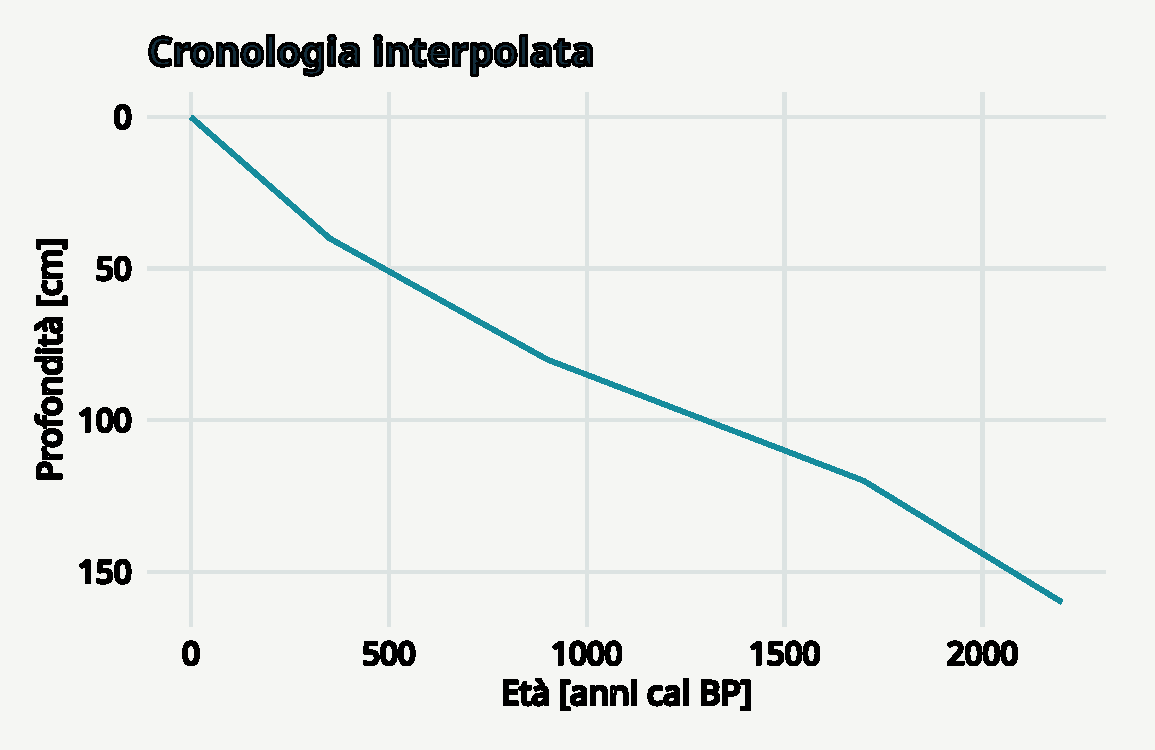
\includegraphics[width=\linewidth,height=6.0cm,keepaspectratio]{Esperimenti/m13-interpolazione-A.pdf}\par}
\PSmall{Profondità da interrogare [cm]: 70. Seme: 17.}
}};
\node[anchor=north west,inner sep=0] at([xshift=10.85cm,yshift=-2.12cm]current page.north west){\Colonna{8.16cm}{\PLabel{Scenario A · simulazione}
\PBody{L’interpolazione lineare ricostruisce le età comprese fra due ancore mediante pesi determinati dalla profondità relativa. Nel modello sintetico, ciascun segmento assume un tasso apparente costante, mentre il passaggio a un segmento successivo può cambiarlo. Il controllo consente di interrogare una profondità e confrontarne l’età con la forma della cronologia.}
\par\smallskip{\centering\adjustbox{max width=.98\linewidth}{$\displaystyle t(z)=t_i+\frac{z-z_i}{z_{i+1}-z_i}(t_{i+1}-t_i),\quad r_i=\frac{\Delta z_i}{\Delta t_i}$}\par\smallskip}
\PSmall{z è la profondità richiesta; $z_i$ e $t_i$ sono profondità ed età delle ancore. $r_i$ è il rapporto fra incremento di profondità e incremento di età; la conversione da centimetri a millimetri moltiplica il tasso per dieci.}
}};
\node[anchor=north east,inner sep=0] at([xshift=17.1cm,yshift=-12.04cm]current page.north west){\fontsize{7.7}{9}\selectfont \href{https://marzione00.github.io/Lab_Geo/\#laboratorio/m13-interpolazione}{\color{Classical}\bfseries Apri il laboratorio · m13-interpolazione}};
\end{tikzpicture}\end{frame}

\begin{frame}[plain]\hypertarget{slide21}{}
\bookmark[level=1,page=21]{Confronto | Interpolazione e tassi di accumulo}
\begin{tikzpicture}[remember picture,overlay]
\PilotChrome{Confronto | Interpolazione e tassi di accumulo}{INTERPOLAZIONE E TASSI DI ACCUMULO}{21}{L’interpolazione lineare assume un tasso costante entro ciascun intervallo fra ancore.}
\node[anchor=north west,inner sep=0] at([xshift=.96cm,yshift=-2.12cm]current page.north west){\Colonna{9.40cm}{{\centering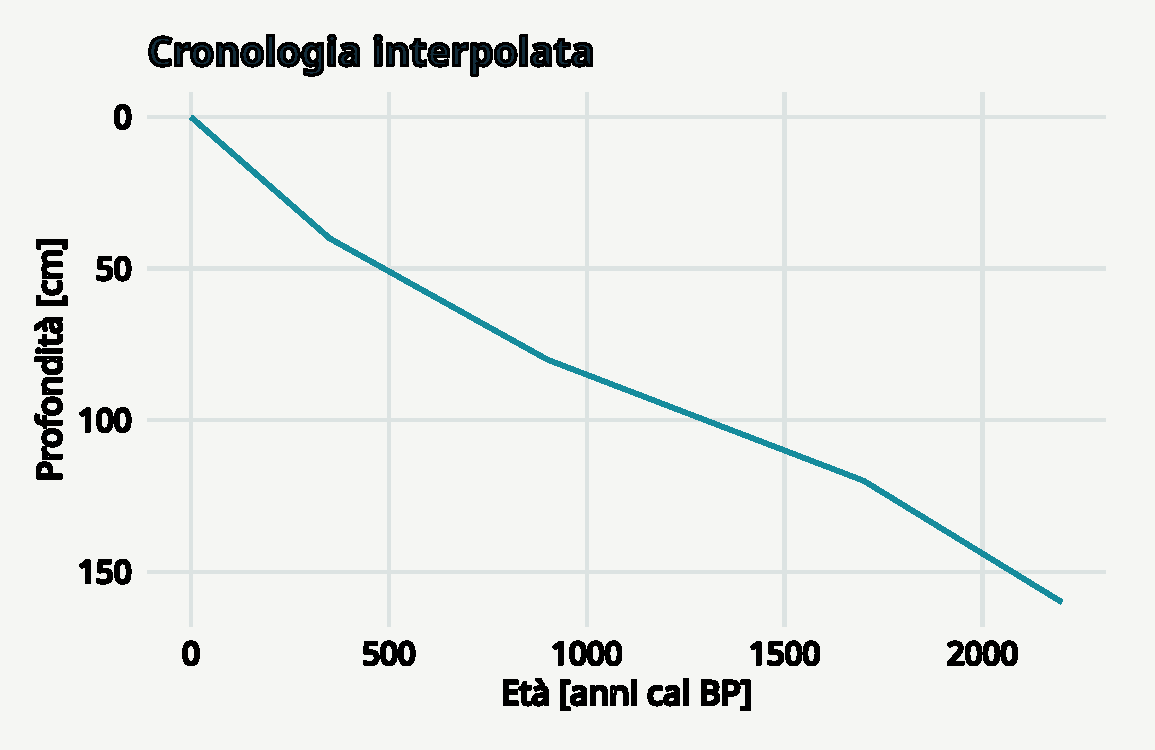
\includegraphics[width=\linewidth,height=5.6cm,keepaspectratio]{Esperimenti/m13-interpolazione-B.pdf}\par}
\PSmall{Profondità da interrogare [cm]: 70 $\to$ 140. Tutti gli altri parametri e il seme sono fissi.}
}};
\node[anchor=north west,inner sep=0] at([xshift=10.85cm,yshift=-2.12cm]current page.north west){\Colonna{8.16cm}{\PLabel{Confronto fra gli scenari}
{\fontsize{10.2}{12.8}\selectfont\begin{tabular}{@{}>{\raggedright\arraybackslash}p{0.48\linewidth}@{\hspace{.13cm}}>{\raggedright\arraybackslash}p{0.224\linewidth}@{\hspace{.13cm}}>{\raggedright\arraybackslash}p{0.224\linewidth}@{}}\toprule Grandezza & A & B\\[2.3pt]
\midrule 
Età richiesta & 762 & 1950\\[2.3pt]
Tasso minimo [mm/anno] & 0,5 & 0,5\\[2.3pt]
Tasso massimo [mm/anno] & 1,14 & 1,14\\[2.3pt]
\bottomrule\end{tabular}\par}
\vspace{.25cm}\PBody{Nel profilo del simulatore, interrogare 140 cm anziché 70 cambia l’età interpolata. I tassi dei segmenti restano gli stessi perché le ancore sono fisse.}
}};
\node[anchor=north east,inner sep=0] at([xshift=17.1cm,yshift=-12.04cm]current page.north west){\fontsize{7.7}{9}\selectfont \href{https://marzione00.github.io/Lab_Geo/\#laboratorio/m13-interpolazione}{\color{Classical}\bfseries Apri il laboratorio · m13-interpolazione}};
\end{tikzpicture}\end{frame}

\begin{frame}[plain]\hypertarget{slide22}{}
\bookmark[level=0,page=22]{Scenari cronologici e propagazione}
\bookmark[level=1,page=22]{Due ancore incerte producono un’età incerta}
\begin{tikzpicture}[remember picture,overlay]
\PilotChrome{Due ancore incerte producono un’età incerta}{SCENARI CRONOLOGICI E PROPAGAZIONE}{22}{Per propagare l’incertezza occorrono pesi e covarianze.}
\node[anchor=north west,inner sep=0] at([xshift=.96cm,yshift=-2.12cm]current page.north west){\Colonna{9.40cm}{\PLabel{Domanda}
\PBody{Le deviazioni standard delle età ai lati del livello sono 25 e 40 anni. Consideriamo prima errori indipendenti e poi una correlazione positiva.}
\vspace{.35cm}\PLabel{Interpretazione}
\PBody{Con pesi uguali, una covarianza positiva allarga l’incertezza dell’età interpolata. Il confronto cambia solo la dipendenza tra le ancore.}
}};
\node[anchor=north west,inner sep=0] at([xshift=10.85cm,yshift=-2.12cm]current page.north west){\Colonna{8.16cm}{\begin{tcolorbox}[enhanced,arc=1.7mm,boxrule=.6pt,colback=white,colframe=Classical!60!Navy,colbacktitle=Navy,coltitle=white,fonttitle=\bfseries\small,title={R · calcolo riproducibile},left=1.7mm,right=1.3mm,top=1.1mm,bottom=1.1mm,before skip=1mm,after skip=1.0mm]\lstinputlisting[style=GeoR,language=R]{Codice/capitolo-03.R}\end{tcolorbox}
\PLabel{Risultato in R}
\begin{tcolorbox}[colback=GeoTint,colframe=Rule,boxrule=.5pt,arc=1.4mm,left=2mm,right=1mm,top=1mm,bottom=1mm]{\fontsize{9}{12}\selectfont\ttfamily \mbox{[1]\ 23.6\ 29.3}}\end{tcolorbox}}};
\end{tikzpicture}\end{frame}

\begin{frame}[plain]\hypertarget{slide23}{}
\bookmark[level=1,page=23]{Perturbazioni delle ancore e modello di sensibilità}
\begin{tikzpicture}[remember picture,overlay]
\PilotChrome{Perturbazioni delle ancore e modello di sensibilità}{SCENARI CRONOLOGICI E PROPAGAZIONE}{23}{La distribuzione degli scenari è definita dalle ipotesi sulle perturbazioni.}
\node[anchor=north west,inner sep=0] at([xshift=.96cm,yshift=-2.12cm]current page.north west){\Colonna{9.40cm}{{\centering\resizebox{.97\linewidth}{!}{\begin{tikzpicture}[x=1cm,y=-.87cm,every node/.style={font=\fontsize{12.2}{15}\selectfont,text=Ink},arr/.style={-{Stealth[length=2mm]},line width=.8pt,draw=Classical}]\path[use as bounding box] (0,0) rectangle (7.45,6.2);
\draw[draw=Classical,fill=Classical!8,rounded corners=2pt,line width=.7pt] (0.5,0.7) rectangle (6.9,1.9);
\node[anchor=center,text=Ink,font=\fontsize{11}{15}\selectfont,text width=6cm,align=center] at (3.7,1.3) {Ancore e deviazioni standard ipotizzate};
\draw[arr,draw=Classical] (3.7,2.1)--(3.7,2.6);
\draw[draw=Quantum,fill=Quantum!8,rounded corners=2pt,line width=.7pt] (0.5,2.8) rectangle (6.9,4);
\node[anchor=center,text=Ink,font=\fontsize{12.2}{15}\selectfont,text width=6cm,align=center] at (3.7,3.4) {500 vettori di età perturbate};
\draw[arr,draw=Classical] (3.7,4.2)--(3.7,4.7);
\node[anchor=center,text=Ink,font=\fontsize{11}{15}\selectfont,text width=6.5cm,align=center] at (3.7,5.3) {Controllo di monotonicità per ogni vettore};

\end{tikzpicture}}\par}
\PSmall{i: ancora; b: scenario; $t_i$: età di base; $\sigma_i$: deviazione prescelta. Indipendenza prima del controllo di monotonicità.}
}};
\node[anchor=north west,inner sep=0] at([xshift=10.85cm,yshift=-2.12cm]current page.north west){\Colonna{8.16cm}{\PBody{Gli scenari aggiungono alle età di base perturbazioni gaussiane con deviazioni standard didattiche pari a 0, 25, 40, 55, 80 e 100 anni. Le perturbazioni delle diverse ancore sono assunte indipendenti prima dell’eventuale condizionamento alla monotonicità; la prima ancora rimane fissa. Questa costruzione quantifica la sensibilità alle ipotesi prescelte e non equivale alla stima di una cronologia bayesiana da datazioni reali. Seme e sequenza dei numeri casuali vengono conservati per rendere identico il confronto fra procedure.}
\par\smallskip{\centering\adjustbox{max width=.98\linewidth}{$\displaystyle T_i^{(b)}=t_i+\sigma_i E_i^{(b)},\qquad E_i^{(b)}\overset{\rm iid}{\sim}N(0,1)$}\par\smallskip}
}};
\end{tikzpicture}\end{frame}

\begin{frame}[plain]\hypertarget{slide24}{}
\bookmark[level=1,page=24]{Monotonicità e identità delle ancore}
\begin{tikzpicture}[remember picture,overlay]
\PilotChrome{Monotonicità e identità delle ancore}{SCENARI CRONOLOGICI E PROPAGAZIONE}{24}{Un vincolo di ordine deve essere applicato senza trasferire un’età da una profondità all’altra.}
\node[anchor=north west,inner sep=0] at([xshift=.96cm,yshift=-2.12cm]current page.north west){\Colonna{9.40cm}{\begin{tcolorbox}[enhanced,arc=1.7mm,boxrule=.6pt,colback=white,colframe=Classical!60!Navy,colbacktitle=Navy,coltitle=white,fonttitle=\bfseries\small,title={R · procedura},left=1.7mm,right=1.3mm,top=1.1mm,bottom=1.1mm,before skip=1mm,after skip=1.0mm]\lstinputlisting[style=GeoR,language=R]{Codice/lettura-12.R}\end{tcolorbox}
}};
\node[anchor=north west,inner sep=0] at([xshift=10.85cm,yshift=-2.12cm]current page.north west){\Colonna{8.16cm}{\PBody{Il controllo esamina ogni vettore di età mantenendo l’associazione con le profondità originarie. Uno scenario non monotono viene escluso esplicitamente, mentre ordinare le età lo trasformerebbe in una configurazione diversa da quella generata. Il rifiuto condiziona la distribuzione delle perturbazioni e può introdurre dipendenza fra ancore. Con i valori e la sequenza inclusi, tutti i cinquecento scenari superano il controllo; il codice mantiene comunque la verifica, che diventa sostanziale aumentando le deviazioni standard o riducendo la separazione temporale delle ancore.}
}};
\end{tikzpicture}\end{frame}

\begin{frame}[plain]\hypertarget{slide25}{}
\bookmark[level=1,page=25]{Bande puntuali del modello età–profondità}
\begin{tikzpicture}[remember picture,overlay]
\PilotChrome{Bande puntuali del modello età–profondità}{SCENARI CRONOLOGICI E PROPAGAZIONE}{25}{Una banda deve dichiarare quali fonti di incertezza siano state propagate e quali restino escluse.}
\node[anchor=north west,inner sep=0] at([xshift=.96cm,yshift=-2.12cm]current page.north west){\Colonna{9.40cm}{{\centering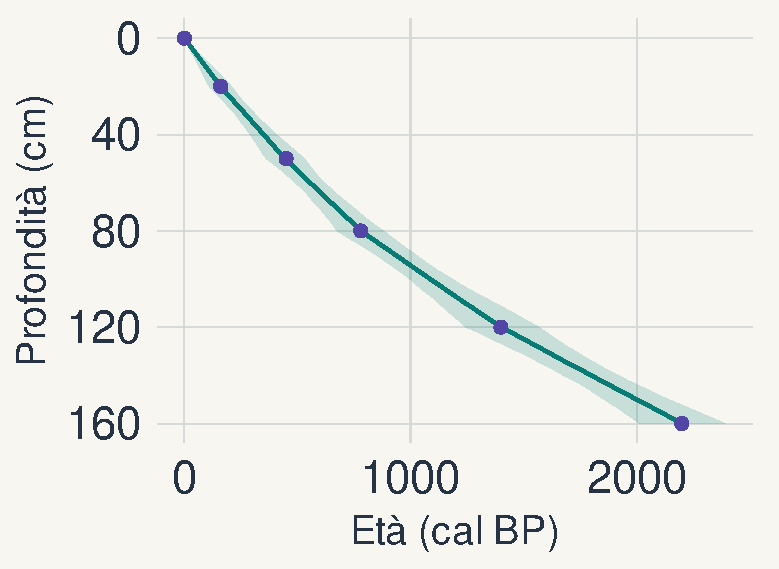
\includegraphics[width=\linewidth,height=6.15cm,keepaspectratio]{Figure/F03.pdf}\par}
\PSmall{Mediana e quantili puntuali degli scenari monotoni. Le ancore di base sono indicate in viola.}
}};
\node[anchor=north west,inner sep=0] at([xshift=10.85cm,yshift=-2.12cm]current page.north west){\Colonna{8.16cm}{\PBody{Ogni scenario accettato viene interpolato sulle medesime profondità e produce una curva cronologica completa. I quantili al 2,5\%, 50\% e 97,5\% vengono calcolati separatamente a ogni profondità, definendo una banda puntuale degli scenari. Tale banda esprime la variabilità indotta dalle perturbazioni specificate; non possiede automaticamente una copertura frequentista certificata né una probabilità simultanea per l’intera curva. L’incertezza sulla forma fra le ancore rimane esclusa quando tutti gli scenari utilizzano la medesima interpolazione lineare.}
}};
\end{tikzpicture}\end{frame}

\begin{frame}[plain]\hypertarget{slide26}{}
\bookmark[level=1,page=26]{Distribuzione dell’età a una profondità prefissata}
\begin{tikzpicture}[remember picture,overlay]
\PilotChrome{Distribuzione dell’età a una profondità prefissata}{SCENARI CRONOLOGICI E PROPAGAZIONE}{26}{I quantili descrivono gli scenari adottati e non aggiungono nuove evidenze di datazione.}
\node[anchor=north west,inner sep=0] at([xshift=.96cm,yshift=-2.12cm]current page.north west){\Colonna{9.40cm}{{\centering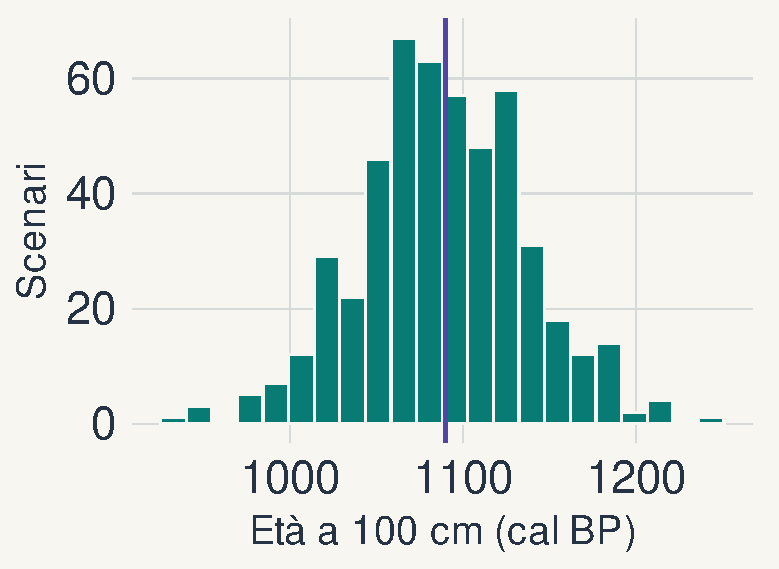
\includegraphics[width=\linewidth,height=6.15cm,keepaspectratio]{Figure/F04.pdf}\par}
\PSmall{Età a 100 centimetri nei cinquecento scenari. La linea viola indica la cronologia di base.}
}};
\node[anchor=north west,inner sep=0] at([xshift=10.85cm,yshift=-2.12cm]current page.north west){\Colonna{8.16cm}{\PBody{A cento centimetri, la cronologia di base assegna 1090 anni cal BP, combinando con pesi uguali le ancore a ottanta e centoventi centimetri. La distribuzione degli scenari restituisce una mediana prossima a 1087,5 anni e quantili al 2,5\% e 97,5\% prossimi a 997,7 e 1186,5 anni. Le differenze fra sintesi Monte Carlo e valore di base riflettono la sequenza finita delle perturbazioni. Raddoppiare le deviazioni standard definirebbe una nuova analisi di sensibilità, della quale andrebbero riportati anche gli eventuali scenari esclusi.}
\par\smallskip{\centering\adjustbox{max width=.98\linewidth}{$\displaystyle T(100)=\tfrac12T(80)+\tfrac12T(120)$}\par\smallskip}
}};
\end{tikzpicture}\end{frame}

\begin{frame}[plain]\hypertarget{slide27}{}
\bookmark[level=1,page=27]{Propagazione lineare e covarianza fra età}
\begin{tikzpicture}[remember picture,overlay]
\PilotChrome{Propagazione lineare e covarianza fra età}{SCENARI CRONOLOGICI E PROPAGAZIONE}{27}{La propagazione deve conservare la dipendenza indotta dalle ancore comuni.}
\node[anchor=north west,inner sep=0] at([xshift=.96cm,yshift=-2.12cm]current page.north west){\Colonna{9.40cm}{{\centering\resizebox{.97\linewidth}{!}{\begin{tikzpicture}[x=1cm,y=-.87cm,every node/.style={font=\fontsize{12.2}{15}\selectfont,text=Ink},arr/.style={-{Stealth[length=2mm]},line width=.8pt,draw=Classical}]\path[use as bounding box] (0,0) rectangle (7.45,6.2);
\node[anchor=center,text=Ink,font=\fontsize{12.2}{15}\selectfont,text width=6cm,align=center] at (3.7,0.7) {Ancora condivisa};
\fill[Quantum] (3.7,2) circle (4pt);\draw[arr,draw=Classical] (3.3,2.3)--(1.7,3.6);
\draw[arr,draw=Classical] (4.1,2.3)--(5.7,3.6);
\draw[draw=Classical,fill=Classical!8,rounded corners=2pt,line width=.7pt] (0.5,3.8) rectangle (3,5.1);
\draw[draw=Quantum,fill=Quantum!8,rounded corners=2pt,line width=.7pt] (4.4,3.8) rectangle (6.9,5.1);
\node[anchor=center,text=Ink,font=\fontsize{16}{15}\selectfont] at (1.75,4.45) {$T(z_1)$};
\node[anchor=center,text=Ink,font=\fontsize{16}{15}\selectfont] at (5.65,4.45) {$T(z_2)$};
\node[anchor=center,text=Ink,font=\fontsize{11}{15}\selectfont,text width=6.8cm,align=center] at (3.7,5.8) {Le due età ereditano una perturbazione comune.};

\end{tikzpicture}}\par}
\PSmall{T: vettore delle sei età; w(z): pesi d’interpolazione alla profondità z; $\Sigma$: covarianza delle ancore. Le età derivate condividono i pesi.}
}};
\node[anchor=north west,inner sep=0] at([xshift=10.85cm,yshift=-2.12cm]current page.north west){\Colonna{8.16cm}{\PBody{Entro la medesima specificazione lineare, l’età a una profondità può essere scritta come combinazione delle età delle ancore. La varianza si ricava mediante i pesi di interpolazione e la matrice di covarianza delle ancore. Due profondità possono condividere una o più ancore, producendo covarianza positiva anche quando le perturbazioni delle ancore sono inizialmente indipendenti. Il condizionamento alla monotonicità può modificare la covarianza, richiedendone un aggiornamento coerente.}
\par\smallskip{\centering\adjustbox{max width=.98\linewidth}{$\displaystyle T(z)=w(z)^\top T,\qquad\operatorname{Var}[T(z)]=w(z)^\top\Sigma w(z)$}\par\smallskip}

\par\smallskip{\centering\adjustbox{max width=.98\linewidth}{$\displaystyle \operatorname{Cov}[T(z_1),T(z_2)]=w(z_1)^\top\Sigma w(z_2)$}\par\smallskip}
}};
\end{tikzpicture}\end{frame}

\begin{frame}[plain]\hypertarget{slide28}{}
\bookmark[level=1,page=28]{La monotonicità si controlla scenario per scenario}
\begin{tikzpicture}[remember picture,overlay]
\PilotChrome{La monotonicità si controlla scenario per scenario}{SCENARI CRONOLOGICI E PROPAGAZIONE}{28}{In questa simulazione R6 tutti i 500 scenari superano il controllo.}
\node[anchor=north west,inner sep=0] at([xshift=.96cm,yshift=-2.12cm]current page.north west){\Colonna{9.40cm}{\PLabel{Risultati del caso R6}
{\fontsize{10.2}{12.8}\selectfont\begin{tabular}{@{}>{\raggedright\arraybackslash}p{0.52\linewidth}@{\hspace{.13cm}}>{\raggedright\arraybackslash}p{0.39\linewidth}@{}}\toprule Grandezza & Valore\\[2.3pt]
\midrule 
generati & 500\\[2.3pt]
accettati & 500\\[2.3pt]
scartati & 0\\[2.3pt]
\bottomrule\end{tabular}\par}
}};
\node[anchor=north west,inner sep=0] at([xshift=10.85cm,yshift=-2.12cm]current page.north west){\Colonna{8.16cm}{\PBody{Quante delle cronologie perturbate sono compatibili con l’ordine delle ancore?}
\vspace{.4cm}\PInfo{In questa simulazione R6 tutti i 500 scenari superano il controllo. Modificando le deviazioni standard può cambiare il numero di scenari che soddisfano il vincolo.}
}};
\node[anchor=north east,inner sep=0] at([xshift=17.1cm,yshift=-12.04cm]current page.north west){\fontsize{7.7}{9}\selectfont \href{https://github.com/marzione00/Lab_Geo/blob/649f7cc577b96bd1044d81e78a2f530813e4f96b/materiali/laboratori/M13/M13_N08.R}{\color{Classical}\bfseries Script R · M13\_N08}};
\end{tikzpicture}\end{frame}

\begin{frame}[plain]\hypertarget{slide29}{}
\bookmark[level=1,page=29]{A cento centimetri l’età diventa una distribuzione}
\begin{tikzpicture}[remember picture,overlay]
\PilotChrome{A cento centimetri l’età diventa una distribuzione}{SCENARI CRONOLOGICI E PROPAGAZIONE}{29}{La mediana ricostruita è prossima all’età di base di 1090 anni.}
\node[anchor=north west,inner sep=0] at([xshift=.96cm,yshift=-2.12cm]current page.north west){\Colonna{9.40cm}{\PLabel{Risultati del caso R6}
{\fontsize{10.2}{12.8}\selectfont\begin{tabular}{@{}>{\raggedright\arraybackslash}p{0.44\linewidth}@{\hspace{.13cm}}>{\raggedright\arraybackslash}p{0.48\linewidth}@{}}\toprule Probabilità & Età (cal BP)\\[2.3pt]
\midrule 
0,025 & 997,74\\[2.3pt]
0,5 & 1087,5\\[2.3pt]
0,975 & 1186,5\\[2.3pt]
\bottomrule\end{tabular}\par}
}};
\node[anchor=north west,inner sep=0] at([xshift=10.85cm,yshift=-2.12cm]current page.north west){\Colonna{8.16cm}{\PBody{Quanto si sposta l’età a profondità fissa quando cambiano le ancore?}
\vspace{.4cm}\PInfo{La mediana ricostruita è prossima all’età di base di 1090 anni. I quantili descrivono gli scenari generati sotto le incertezze assegnate alle ancore.}
}};
\node[anchor=north east,inner sep=0] at([xshift=17.1cm,yshift=-12.04cm]current page.north west){\fontsize{7.7}{9}\selectfont \href{https://github.com/marzione00/Lab_Geo/blob/649f7cc577b96bd1044d81e78a2f530813e4f96b/materiali/laboratori/M13/M13_N09.R}{\color{Classical}\bfseries Script R · M13\_N09}};
\end{tikzpicture}\end{frame}

\begin{frame}[plain]\hypertarget{slide30}{}
\bookmark[level=1,page=30]{Scenari cronologici e propagazione}
\begin{tikzpicture}[remember picture,overlay]
\PilotChrome{Scenari cronologici e propagazione}{SCENARI CRONOLOGICI E PROPAGAZIONE}{30}{Costruire cronologie perturbate conservando l’associazione fra età e profondità.}
\node[anchor=north west,inner sep=0] at([xshift=.96cm,yshift=-2.12cm]current page.north west){\Colonna{9.40cm}{{\centering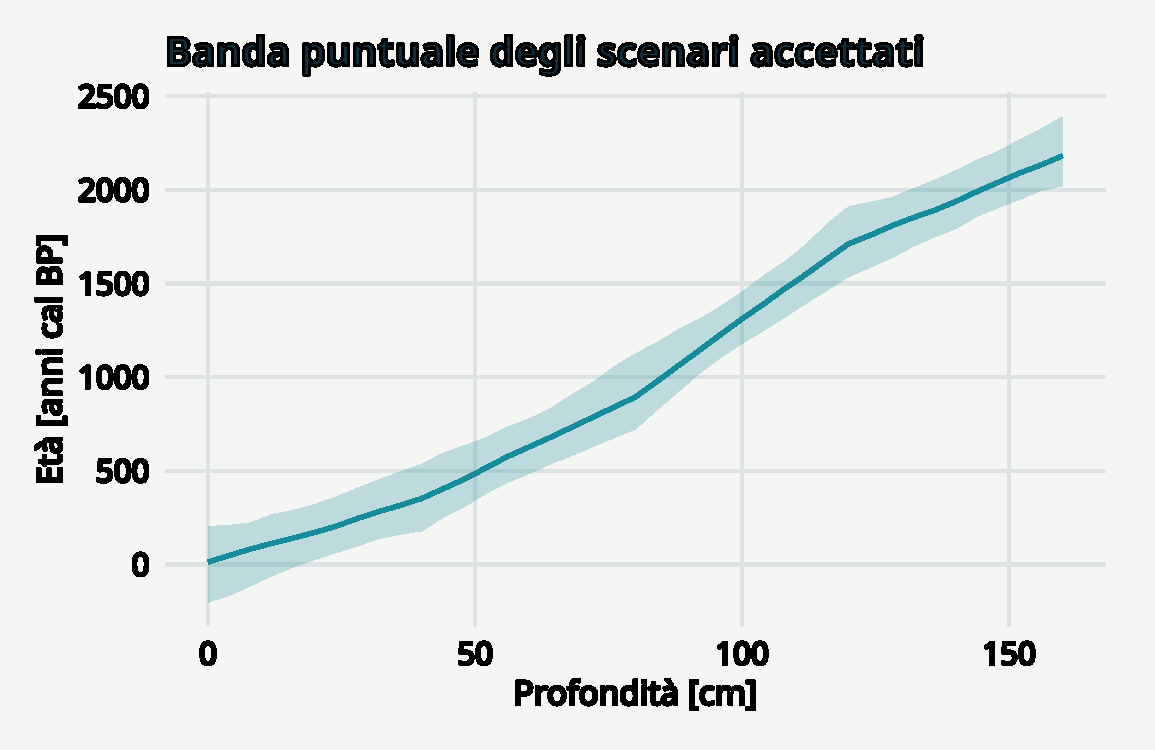
\includegraphics[width=\linewidth,height=6.0cm,keepaspectratio]{Esperimenti/m13-incertezza-A.pdf}\par}
\PSmall{SD delle ancore [anni]: 100. Seme: 17.}
}};
\node[anchor=north west,inner sep=0] at([xshift=10.85cm,yshift=-2.12cm]current page.north west){\Colonna{8.16cm}{\PLabel{Scenario A · simulazione}
\PBody{L’incertezza delle ancore si propaga alle età interpolate perché ciascuna previsione combina le datazioni circostanti. L’esperimento perturba tutte le cinque ancore, compresa quella superficiale, mediante errori gaussiani indipendenti con deviazione standard comune. Ogni configurazione conserva l’associazione fra età e profondità e viene accettata soltanto quando le età rimangono strettamente crescenti.}
\par\smallskip{\centering\adjustbox{max width=.98\linewidth}{$\displaystyle t_b(z)=\operatorname{interp}\{(z_i,t_{i,b})\}$}\par\smallskip}
\PSmall{$z_i$ indica la profondità dell’ancora i e $t_{i,b}$ la sua età nella replica b. $t_b$(z) è la cronologia ottenuta interpolando le ancore della stessa replica; la dispersione controllata è espressa in anni.}
}};
\node[anchor=north east,inner sep=0] at([xshift=17.1cm,yshift=-12.04cm]current page.north west){\fontsize{7.7}{9}\selectfont \href{https://marzione00.github.io/Lab_Geo/\#laboratorio/m13-incertezza}{\color{Classical}\bfseries Apri il laboratorio · m13-incertezza}};
\end{tikzpicture}\end{frame}

\begin{frame}[plain]\hypertarget{slide31}{}
\bookmark[level=1,page=31]{Confronto | Scenari cronologici e propagazione}
\begin{tikzpicture}[remember picture,overlay]
\PilotChrome{Confronto | Scenari cronologici e propagazione}{SCENARI CRONOLOGICI E PROPAGAZIONE}{31}{La selezione degli scenari monotoni condiziona la distribuzione delle cronologie accettate.}
\node[anchor=north west,inner sep=0] at([xshift=.96cm,yshift=-2.12cm]current page.north west){\Colonna{9.40cm}{{\centering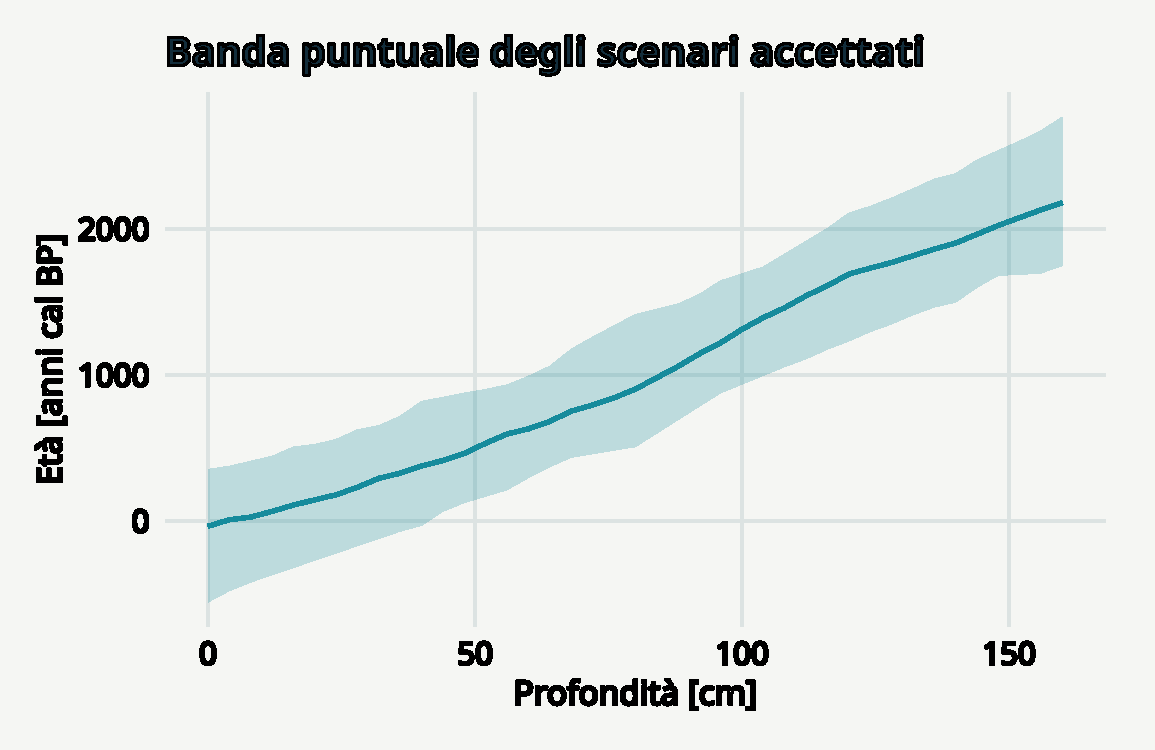
\includegraphics[width=\linewidth,height=5.6cm,keepaspectratio]{Esperimenti/m13-incertezza-B.pdf}\par}
\PSmall{SD delle ancore [anni]: 100 $\to$ 300. Tutti gli altri parametri e il seme sono fissi.}
}};
\node[anchor=north west,inner sep=0] at([xshift=10.85cm,yshift=-2.12cm]current page.north west){\Colonna{8.16cm}{\PLabel{Confronto fra gli scenari}
{\fontsize{10.2}{12.8}\selectfont\begin{tabular}{@{}>{\raggedright\arraybackslash}p{0.48\linewidth}@{\hspace{.13cm}}>{\raggedright\arraybackslash}p{0.224\linewidth}@{\hspace{.13cm}}>{\raggedright\arraybackslash}p{0.224\linewidth}@{}}\toprule Grandezza & A & B\\[2.3pt]
\midrule 
Scenari generati & 200 & 200\\[2.3pt]
Accettati & 199 & 121\\[2.3pt]
Rifiutati & 1 & 79\\[2.3pt]
Ampiezza mediana banda [anni] & 318 & 812\\[2.3pt]
\bottomrule\end{tabular}\par}
\vspace{.25cm}\PBody{Con deviazione standard 300 anni le cronologie accettate scendono a 121 su 200. Anche dopo il controllo di monotonicità le bande si allargano.}
}};
\node[anchor=north east,inner sep=0] at([xshift=17.1cm,yshift=-12.04cm]current page.north west){\fontsize{7.7}{9}\selectfont \href{https://marzione00.github.io/Lab_Geo/\#laboratorio/m13-incertezza}{\color{Classical}\bfseries Apri il laboratorio · m13-incertezza}};
\end{tikzpicture}\end{frame}

\begin{frame}[plain]\hypertarget{slide32}{}
\bookmark[level=0,page=32]{Proxy e risoluzione temporale}
\bookmark[level=1,page=32]{Due centimetri non valgono sempre gli stessi anni}
\begin{tikzpicture}[remember picture,overlay]
\PilotChrome{Due centimetri non valgono sempre gli stessi anni}{PROXY E RISOLUZIONE TEMPORALE}{32}{La risoluzione dipende dal prodotto fra passo di campionamento e pendenza locale.}
\node[anchor=north west,inner sep=0] at([xshift=.96cm,yshift=-2.12cm]current page.north west){\Colonna{9.40cm}{\PLabel{Domanda}
\PBody{Il proxy si misura ogni 2 cm. Nel tratto 0–20 cm passano 160 anni, nel tratto 120–160 cm ne passano 800. Qual è la risoluzione temporale locale?}
\vspace{.35cm}\PLabel{Interpretazione}
\PBody{Il primo tratto dà 16 anni ogni due centimetri, l’ultimo 40. La stessa frequenza di prelievo in profondità lascia intervalli temporali diversi.}
}};
\node[anchor=north west,inner sep=0] at([xshift=10.85cm,yshift=-2.12cm]current page.north west){\Colonna{8.16cm}{\begin{tcolorbox}[enhanced,arc=1.7mm,boxrule=.6pt,colback=white,colframe=Classical!60!Navy,colbacktitle=Navy,coltitle=white,fonttitle=\bfseries\small,title={R · calcolo riproducibile},left=1.7mm,right=1.3mm,top=1.1mm,bottom=1.1mm,before skip=1mm,after skip=1.0mm]\lstinputlisting[style=GeoR,language=R]{Codice/capitolo-04.R}\end{tcolorbox}
\PLabel{Risultato in R}
\begin{tcolorbox}[colback=GeoTint,colframe=Rule,boxrule=.5pt,arc=1.4mm,left=2mm,right=1mm,top=1mm,bottom=1mm]{\fontsize{9}{12}\selectfont\ttfamily \mbox{[1]\ 16\ 40}}\end{tcolorbox}}};
\end{tikzpicture}\end{frame}

\begin{frame}[plain]\hypertarget{slide33}{}
\bookmark[level=1,page=33]{Il proxy sulla scala della profondità}
\begin{tikzpicture}[remember picture,overlay]
\PilotChrome{Il proxy sulla scala della profondità}{PROXY E RISOLUZIONE TEMPORALE}{33}{La scala della profondità descrive lo spessore dell’archivio e deve essere distinta dalla scala del tempo.}
\node[anchor=north west,inner sep=0] at([xshift=.96cm,yshift=-2.12cm]current page.north west){\Colonna{9.40cm}{{\centering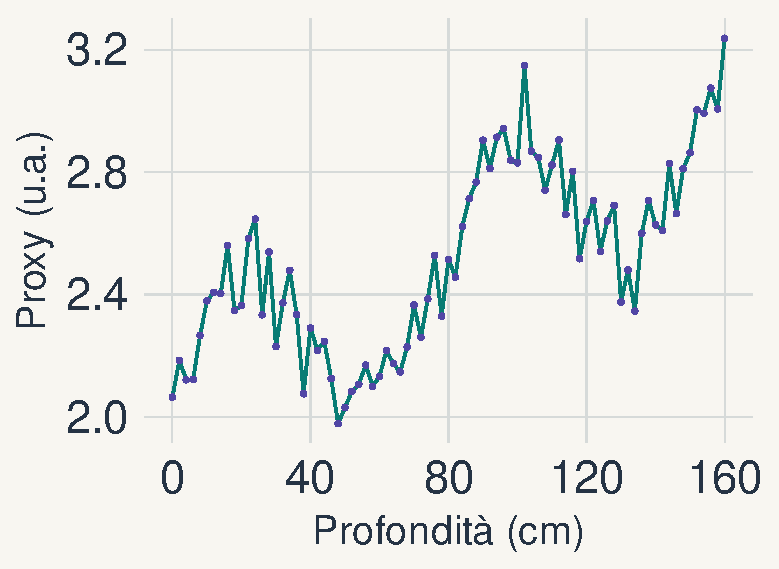
\includegraphics[width=\linewidth,height=6.15cm,keepaspectratio]{Figure/F05.pdf}\par}
\PSmall{Ottantuno osservazioni sintetiche, separate da due centimetri. I punti conservano la posizione dei campioni originari.}
}};
\node[anchor=north west,inner sep=0] at([xshift=10.85cm,yshift=-2.12cm]current page.north west){\Colonna{8.16cm}{\PBody{Il proxy sintetico comprende ottantuno valori acquisiti idealmente a passo costante di due centimetri. Su questa scala, intervalli uguali dell’asse rappresentano spessori uguali, mentre oscillazioni e tendenze descrivono variazioni lungo la successione. La regolarità spaziale consente di riconoscere l’ordine dei campioni, ma lascia aperta la durata rappresentata da ciascun tratto. Prima di collegare un massimo o una variazione a un evento temporale occorre applicare la cronologia e valutarne la risoluzione, insieme al rumore del proxy e al supporto del campione.}
}};
\end{tikzpicture}\end{frame}

\begin{frame}[plain]\hypertarget{slide34}{}
\bookmark[level=1,page=34]{Il medesimo proxy sulla scala del tempo}
\begin{tikzpicture}[remember picture,overlay]
\PilotChrome{Il medesimo proxy sulla scala del tempo}{PROXY E RISOLUZIONE TEMPORALE}{34}{Trasformare l’asse modifica le distanze fra osservazioni e il significato delle procedure temporali.}
\node[anchor=north west,inner sep=0] at([xshift=.96cm,yshift=-2.12cm]current page.north west){\Colonna{9.40cm}{{\centering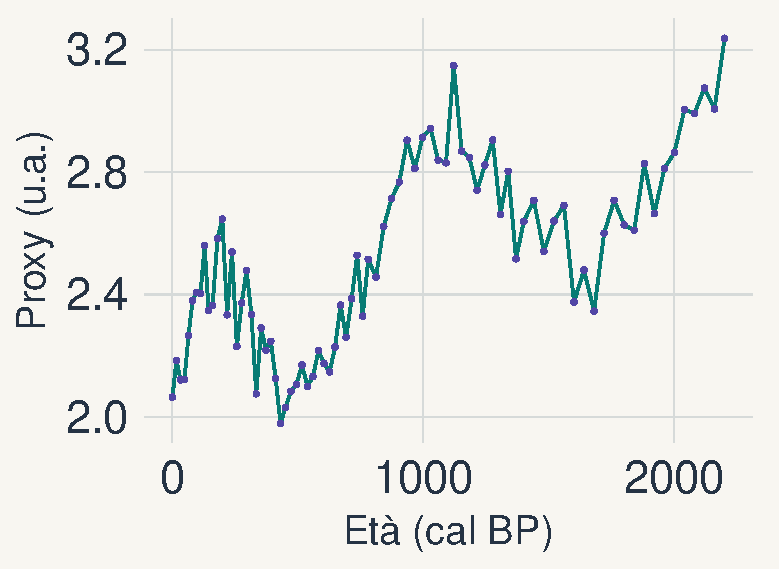
\includegraphics[width=\linewidth,height=6.15cm,keepaspectratio]{Figure/F06.pdf}\par}
\PSmall{Gli stessi ottantuno valori dopo la conversione mediante la cronologia di base. Le distanze temporali sono irregolari.}
}};
\node[anchor=north west,inner sep=0] at([xshift=10.85cm,yshift=-2.12cm]current page.north west){\Colonna{8.16cm}{\PBody{La trasformazione dell’asse assegna un’età a ogni profondità, lasciando invariati i valori del proxy. Poiché i tassi apparenti cambiano fra i segmenti, intervalli uguali in profondità corrispondono a durate diverse e la densità temporale dei campioni varia. Il passo originario di 2 cm corrisponde a 16 anni nel primo segmento e a 40 nell’ultimo, dilatando diversamente i tratti dell’asse. Qualunque analisi che richieda campionamento regolare nel tempo deve quindi verificare il nuovo asse, anziché trasferire automaticamente la frequenza definita in centimetri.}
}};
\end{tikzpicture}\end{frame}

\begin{frame}[plain]\hypertarget{slide35}{}
\bookmark[level=1,page=35]{Passo di campionamento e durata effettiva}
\begin{tikzpicture}[remember picture,overlay]
\PilotChrome{Passo di campionamento e durata effettiva}{PROXY E RISOLUZIONE TEMPORALE}{35}{La risoluzione temporale deve essere valutata localmente lungo l’archivio.}
\node[anchor=north west,inner sep=0] at([xshift=.96cm,yshift=-2.12cm]current page.north west){\Colonna{9.40cm}{{\centering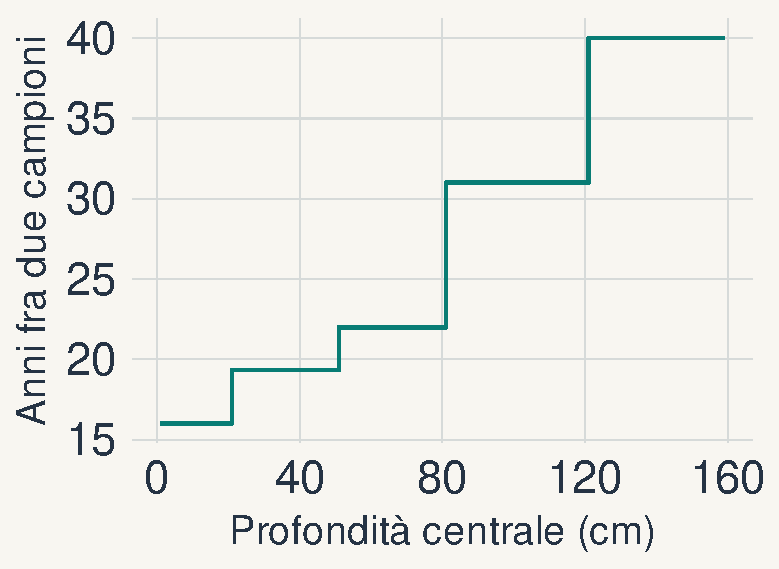
\includegraphics[width=\linewidth,height=6.15cm,keepaspectratio]{Figure/F12.pdf}\par}
\PSmall{Durata fra due campioni adiacenti, rappresentata alla profondità intermedia. Il passo spaziale resta pari a due centimetri.}
}};
\node[anchor=north west,inner sep=0] at([xshift=10.85cm,yshift=-2.12cm]current page.north west){\Colonna{8.16cm}{\PBody{La durata fra due campioni consecutivi dipende dalla pendenza locale della curva età–profondità. Nel laboratorio, il passo di due centimetri rappresenta sedici anni nel primo segmento e quaranta anni nell’ultimo. Una variazione breve può pertanto risultare diversamente risolta lungo la successione, anche se il protocollo di campionamento resta costante in profondità. L’interpolazione cronologica rende esplicita questa eterogeneità, alla quale si aggiungono incertezze delle ancore e durata integrata dal supporto fisico di ciascun campione.}
\par\smallskip{\centering\adjustbox{max width=.98\linewidth}{$\displaystyle \Delta t_i=t(z_{i+1})-t(z_i)$}\par\smallskip}
}};
\end{tikzpicture}\end{frame}

\begin{frame}[plain]\hypertarget{slide36}{}
\bookmark[level=1,page=36]{Finestre per indice e finestre temporali}
\begin{tikzpicture}[remember picture,overlay]
\PilotChrome{Finestre per indice e finestre temporali}{PROXY E RISOLUZIONE TEMPORALE}{36}{L’unità della finestra e i pesi stabiliscono quale variazione venga attenuata.}
\node[anchor=north west,inner sep=0] at([xshift=.96cm,yshift=-2.12cm]current page.north west){\Colonna{9.40cm}{{\centering\resizebox{.97\linewidth}{!}{\begin{tikzpicture}[x=1cm,y=-.87cm,every node/.style={font=\fontsize{12.2}{15}\selectfont,text=Ink},arr/.style={-{Stealth[length=2mm]},line width=.8pt,draw=Classical}]\path[use as bounding box] (0,0) rectangle (7.45,6.2);
\draw[arr,draw=Classical] (0.5,2)--(6.9,2);
\draw[arr,draw=Classical] (0.5,4.2)--(6.9,4.2);
\fill[Classical] (1,2) circle (2.5pt);\fill[Classical] (2.1,2) circle (2.5pt);\fill[Classical] (3.2,2) circle (2.5pt);\fill[Classical] (4.3,2) circle (2.5pt);\fill[Classical] (5.4,2) circle (2.5pt);\fill[Quantum] (1,4.2) circle (2.5pt);\fill[Quantum] (1.7,4.2) circle (2.5pt);\fill[Quantum] (2.5,4.2) circle (2.5pt);\fill[Quantum] (4.1,4.2) circle (2.5pt);\fill[Quantum] (6.1,4.2) circle (2.5pt);\node[anchor=center,text=Ink,font=\fontsize{11}{15}\selectfont,text width=6.5cm,align=center] at (3.7,1.1) {Passo costante in profondità};
\node[anchor=center,text=Ink,font=\fontsize{11}{15}\selectfont,text width=6.5cm,align=center] at (3.7,5.2) {Tempi irregolari dopo la conversione};

\end{tikzpicture}}\par}
\PSmall{$t_0$: età centrale; $t_i$: età assegnata al campione i. La finestra temporale include tutti i campioni entro 100 anni dal centro.}
}};
\node[anchor=north west,inner sep=0] at([xshift=10.85cm,yshift=-2.12cm]current page.north west){\Colonna{8.16cm}{\PBody{Una finestra di cinque campioni copre sempre otto centimetri fra i suoi estremi, mentre la durata cambia con la cronologia. Una finestra di più o meno cento anni mantiene invece un criterio temporale e può contenere un numero diverso di campioni nelle varie porzioni della successione. La media dei punti entro la finestra attribuisce uguale peso ai campioni, mentre una media sul tempo richiederebbe pesi coerenti con gli intervalli rappresentati. Il metodo di smoothing deve quindi specificare ampiezza, unità e regola di ponderazione.}
\par\smallskip{\centering\adjustbox{max width=.98\linewidth}{$\displaystyle \mathcal W_t=\{i:|t_i-t_0|\le100\ \mathrm{anni}\}$}\par\smallskip}
}};
\end{tikzpicture}\end{frame}

\begin{frame}[plain]\hypertarget{slide37}{}
\bookmark[level=1,page=37]{Interpolazione temporale e informazione osservata}
\begin{tikzpicture}[remember picture,overlay]
\PilotChrome{Interpolazione temporale e informazione osservata}{PROXY E RISOLUZIONE TEMPORALE}{37}{La regolarizzazione della griglia temporale modifica la rappresentazione e il modello di dipendenza.}
\node[anchor=north west,inner sep=0] at([xshift=.96cm,yshift=-2.12cm]current page.north west){\Colonna{9.40cm}{\PLabel{Metodo}
\PBody{Ricostruire il proxy ogni dieci anni produce 221 righe, tutte derivate dalle ottantuno misure originarie. La griglia regolare può essere utile per confronti grafici o per procedure che richiedano un asse uniforme, purché si riconoscano la dipendenza introdotta e le ipotesi dell’interpolazione. Il numero delle righe ricostruite non fornisce nuovi gradi di libertà osservativi. Se l’analisi successiva riguarda incertezza o significatività, deve conservare la provenienza dai campioni originali e la variabilità della trasformazione cronologica.}
}};
\node[anchor=north west,inner sep=0] at([xshift=10.85cm,yshift=-2.12cm]current page.north west){\Colonna{8.16cm}{\PLabel{Formalismo}
\par\smallskip{\centering\adjustbox{max width=.98\linewidth}{$\displaystyle \widetilde y(q)=\sum_i a_i(q)y_i$}\par\smallskip}
\PLabel{Interpretazione}
\PBody{q è l’età richiesta; $y_i$ il proxy osservato; $a_i(q)$ il peso del campione i. Nell’interpolazione lineare interna intervengono due vicini, con pesi non negativi che sommano a uno. Più punti ricostruiti possono condividere campioni e ancore cronologiche, introducendo dipendenza su entrambi gli assi.}
}};
\end{tikzpicture}\end{frame}

\begin{frame}[plain]\hypertarget{slide38}{}
\bookmark[level=1,page=38]{Una finestra per punti e una per anni selezionano dati diversi}
\begin{tikzpicture}[remember picture,overlay]
\PilotChrome{{\fontsize{17.3}{19}\selectfont Una finestra per punti e una per anni selezionano dati diversi}}{PROXY E RISOLUZIONE TEMPORALE}{38}{Confronta numero di osservazioni e valore medio.}
\node[anchor=north west,inner sep=0] at([xshift=.96cm,yshift=-2.12cm]current page.north west){\Colonna{9.40cm}{\PLabel{Risultati del caso R6}
{\fontsize{10.2}{12.8}\selectfont\begin{tabular}{@{}>{\raggedright\arraybackslash}p{0.31\linewidth}@{\hspace{.13cm}}>{\raggedright\arraybackslash}p{0.29\linewidth}@{\hspace{.13cm}}>{\raggedright\arraybackslash}p{0.32\linewidth}@{}}\toprule schema & Numero & media\\[2.3pt]
\midrule 
5 punti & 5 & 2,2793\\[2.3pt]
100 anni & 11 & 2,2626\\[2.3pt]
\bottomrule\end{tabular}\par}
}};
\node[anchor=north west,inner sep=0] at([xshift=10.85cm,yshift=-2.12cm]current page.north west){\Colonna{8.16cm}{\PBody{Che cosa accade alla media locale cambiando la definizione di finestra?}
\vspace{.4cm}\PInfo{Confronta numero di osservazioni e valore medio. Due finestre centrate nella stessa regione possono includere livelli diversi perché la scala temporale è irregolare.}
}};
\node[anchor=north east,inner sep=0] at([xshift=17.1cm,yshift=-12.04cm]current page.north west){\fontsize{7.7}{9}\selectfont \href{https://github.com/marzione00/Lab_Geo/blob/649f7cc577b96bd1044d81e78a2f530813e4f96b/materiali/laboratori/M13/M13_N11.R}{\color{Classical}\bfseries Script R · M13\_N11}};
\end{tikzpicture}\end{frame}

\begin{frame}[plain]\hypertarget{slide39}{}
\bookmark[level=1,page=39]{Risoluzione temporale di un proxy}
\begin{tikzpicture}[remember picture,overlay]
\PilotChrome{Risoluzione temporale di un proxy}{PROXY E RISOLUZIONE TEMPORALE}{39}{Confrontare un campionamento uniforme in profondità con il suo supporto temporale.}
\node[anchor=north west,inner sep=0] at([xshift=.96cm,yshift=-2.12cm]current page.north west){\Colonna{9.40cm}{{\centering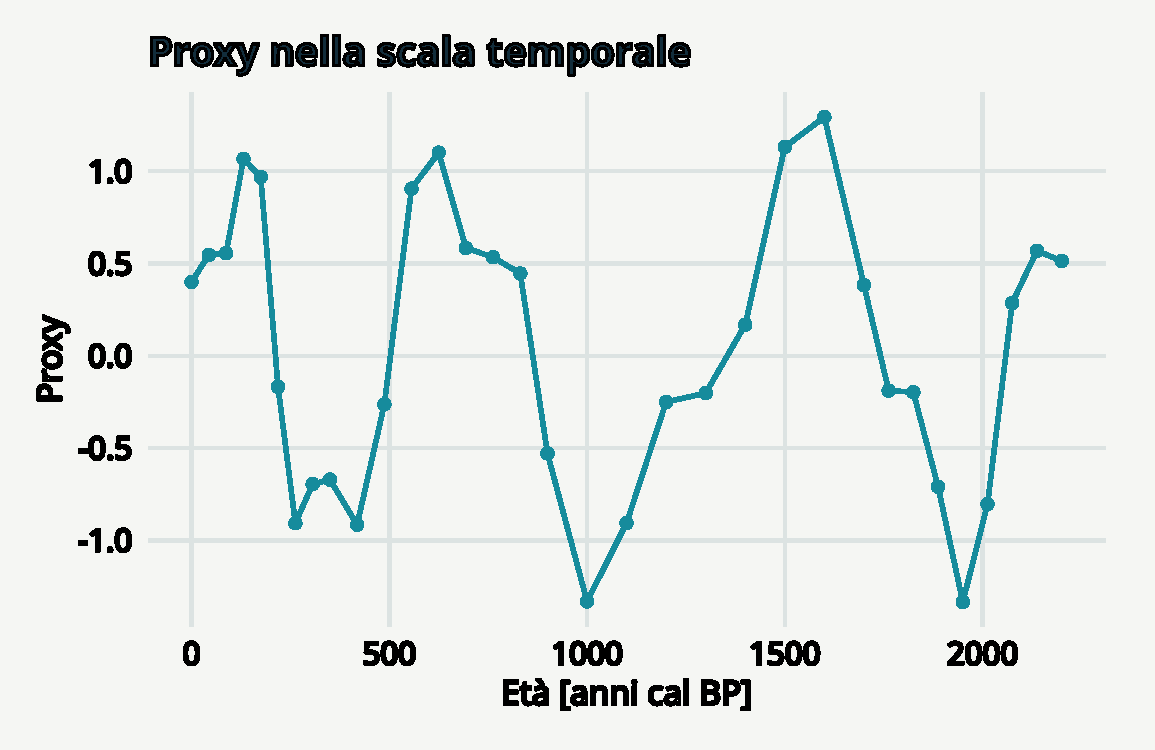
\includegraphics[width=\linewidth,height=6.0cm,keepaspectratio]{Esperimenti/m13-proxy-A.pdf}\par}
\PSmall{Passo in profondità [cm]: 5. Seme: 17.}
}};
\node[anchor=north west,inner sep=0] at([xshift=10.85cm,yshift=-2.12cm]current page.north west){\Colonna{8.16cm}{\PLabel{Scenario A · simulazione}
\PBody{Un campionamento regolare in profondità produce intervalli temporali variabili quando il tasso apparente di accumulo cambia lungo l’archivio. Il proxy sintetico viene osservato a un passo controllabile in centimetri e ciascuna profondità riceve un’età mediante la cronologia a tratti. I punti della figura indicano le osservazioni effettivamente generate, rendendo visibile la loro distribuzione nel tempo.}
\par\smallskip{\centering\adjustbox{max width=.98\linewidth}{$\displaystyle \Delta t_i=t(z_{i+1})-t(z_i)$}\par\smallskip}
\PSmall{$z_i$ e $z_{i+1}$ sono profondità consecutive; t(z) è l’età assegnata dalla cronologia; $\Delta t_i$ è la durata rappresentata dall’intervallo fra i campioni. Il passo in centimetri rimane uniforme, mentre $\Delta t_i$ può variare.}
}};
\node[anchor=north east,inner sep=0] at([xshift=17.1cm,yshift=-12.04cm]current page.north west){\fontsize{7.7}{9}\selectfont \href{https://marzione00.github.io/Lab_Geo/\#laboratorio/m13-proxy}{\color{Classical}\bfseries Apri il laboratorio · m13-proxy}};
\end{tikzpicture}\end{frame}

\begin{frame}[plain]\hypertarget{slide40}{}
\bookmark[level=1,page=40]{Confronto | Risoluzione temporale di un proxy}
\begin{tikzpicture}[remember picture,overlay]
\PilotChrome{Confronto | Risoluzione temporale di un proxy}{PROXY E RISOLUZIONE TEMPORALE}{40}{Una risoluzione costante in profondità può corrispondere a risoluzioni temporali differenti.}
\node[anchor=north west,inner sep=0] at([xshift=.96cm,yshift=-2.12cm]current page.north west){\Colonna{9.40cm}{{\centering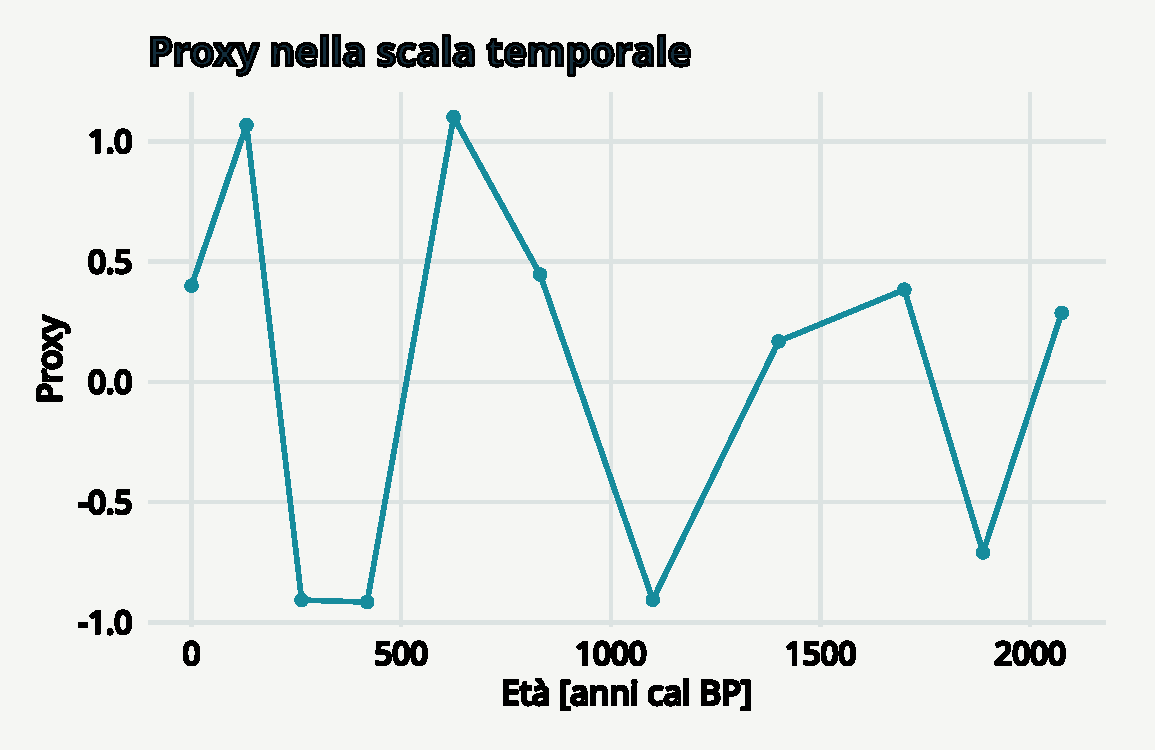
\includegraphics[width=\linewidth,height=5.6cm,keepaspectratio]{Esperimenti/m13-proxy-B.pdf}\par}
\PSmall{Passo in profondità [cm]: 5 $\to$ 15. Tutti gli altri parametri e il seme sono fissi.}
}};
\node[anchor=north west,inner sep=0] at([xshift=10.85cm,yshift=-2.12cm]current page.north west){\Colonna{8.16cm}{\PLabel{Confronto fra gli scenari}
{\fontsize{10.2}{12.8}\selectfont\begin{tabular}{@{}>{\raggedright\arraybackslash}p{0.48\linewidth}@{\hspace{.13cm}}>{\raggedright\arraybackslash}p{0.224\linewidth}@{\hspace{.13cm}}>{\raggedright\arraybackslash}p{0.224\linewidth}@{}}\toprule Grandezza & A & B\\[2.3pt]
\midrule 
Campioni & 33 & 11\\[2.3pt]
Intervallo minimo [anni] & 43,8 & 131\\[2.3pt]
Intervallo massimo [anni] & 100 & 300\\[2.3pt]
\bottomrule\end{tabular}\par}
\vspace{.25cm}\PBody{Il passo triplicato porta da 33 a 11 campioni. La durata massima fra livelli cresce da 100 a 300 anni.}
}};
\node[anchor=north east,inner sep=0] at([xshift=17.1cm,yshift=-12.04cm]current page.north west){\fontsize{7.7}{9}\selectfont \href{https://marzione00.github.io/Lab_Geo/\#laboratorio/m13-proxy}{\color{Classical}\bfseries Apri il laboratorio · m13-proxy}};
\end{tikzpicture}\end{frame}

\begin{frame}[plain]\hypertarget{slide41}{}
\bookmark[level=0,page=41]{Discontinuità e sensibilità del modello}
\bookmark[level=1,page=41]{Una lacuna sposta soltanto il ramo più antico}
\begin{tikzpicture}[remember picture,overlay]
\PilotChrome{Una lacuna sposta soltanto il ramo più antico}{DISCONTINUITÀ E SENSIBILITÀ DEL MODELLO}{41}{Per rappresentare una lacuna disegna due rami e dichiara il salto temporale.}
\node[anchor=north west,inner sep=0] at([xshift=.96cm,yshift=-2.12cm]current page.north west){\Colonna{9.40cm}{\PLabel{Domanda}
\PBody{Introduciamo 400 anni mancanti a 80 cm. Il limite superiore della discontinuità ha età 780 cal BP. Quale età ha il limite inferiore?}
\vspace{.35cm}\PLabel{Interpretazione}
\PBody{Ai due lati della medesima superficie stratigrafica corrispondono due età. Un segmento obliquo attraverso il salto inventerebbe sedimento nell’intervallo mancante.}
}};
\node[anchor=north west,inner sep=0] at([xshift=10.85cm,yshift=-2.12cm]current page.north west){\Colonna{8.16cm}{\begin{tcolorbox}[enhanced,arc=1.7mm,boxrule=.6pt,colback=white,colframe=Classical!60!Navy,colbacktitle=Navy,coltitle=white,fonttitle=\bfseries\small,title={R · calcolo riproducibile},left=1.7mm,right=1.3mm,top=1.1mm,bottom=1.1mm,before skip=1mm,after skip=1.0mm]\lstinputlisting[style=GeoR,language=R]{Codice/capitolo-05.R}\end{tcolorbox}
\PLabel{Risultato in R}
\begin{tcolorbox}[colback=GeoTint,colframe=Rule,boxrule=.5pt,arc=1.4mm,left=2mm,right=1mm,top=1mm,bottom=1mm]{\fontsize{9}{12}\selectfont\ttfamily \mbox{sopra\ sotto\ }\\\mbox{\ \ 780\ \ 1180}}\end{tcolorbox}}};
\end{tikzpicture}\end{frame}

\begin{frame}[plain]\hypertarget{slide42}{}
\bookmark[level=1,page=42]{Hiatus come discontinuità della cronologia}
\begin{tikzpicture}[remember picture,overlay]
\PilotChrome{Hiatus come discontinuità della cronologia}{DISCONTINUITÀ E SENSIBILITÀ DEL MODELLO}{42}{Una lacuna deve essere sostenuta da evidenze indipendenti e rappresentata come discontinuità esplicita.}
\node[anchor=north west,inner sep=0] at([xshift=.96cm,yshift=-2.12cm]current page.north west){\Colonna{9.40cm}{{\centering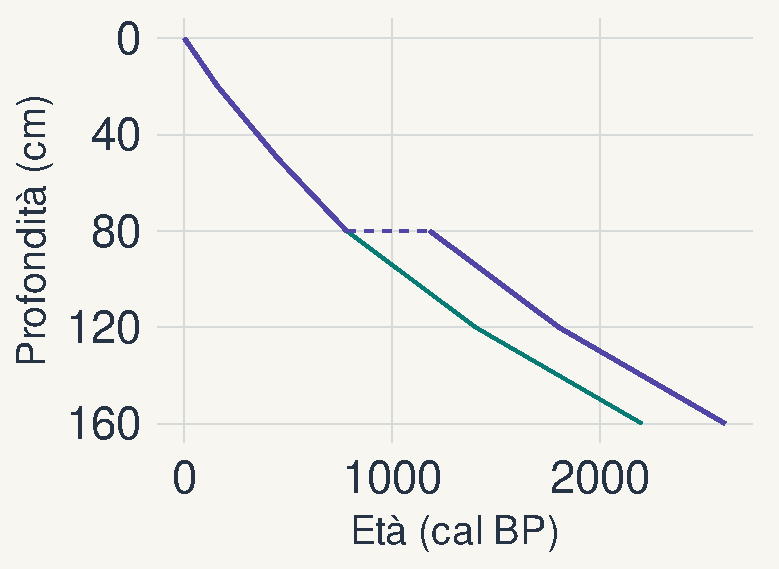
\includegraphics[width=\linewidth,height=6.15cm,keepaspectratio]{Figure/F07.pdf}\par}
\PSmall{Verde: cronologia di base. Viola: scenario con hiatus; il tratteggio indica il salto a 80 centimetri.}
}};
\node[anchor=north west,inner sep=0] at([xshift=10.85cm,yshift=-2.12cm]current page.north west){\Colonna{8.16cm}{\PBody{Lo scenario di hiatus aggiunge quattrocento anni alle profondità superiori a ottanta centimetri, mantenendo separata la cronologia di base. Il salto rappresenta un intervallo temporale privo di sedimentazione conservata nel modello, per il quale servirebbero evidenze stratigrafiche o cronologiche indipendenti. La figura distingue i due rami ai lati della discontinuità, evitando che una linea obliqua suggerisca accumulo attraverso l’intervallo mancante. La scelta della profondità e della durata del salto appartiene allo scenario e non viene inferita automaticamente dal proxy.}
\par\smallskip{\centering\adjustbox{max width=.98\linewidth}{$\displaystyle t_H(z)=t(z)+400\,\mathbf1\{z>80\}$}\par\smallskip}
}};
\end{tikzpicture}\end{frame}

\begin{frame}[plain]\hypertarget{slide43}{}
\bookmark[level=1,page=43]{Inversione cronologica e diagnosi dell’incongruenza}
\begin{tikzpicture}[remember picture,overlay]
\PilotChrome{Inversione cronologica e diagnosi dell’incongruenza}{DISCONTINUITÀ E SENSIBILITÀ DEL MODELLO}{43}{Il controllo riconosce l’incongruenza, mentre la diagnosi richiede evidenze ulteriori.}
\node[anchor=north west,inner sep=0] at([xshift=.96cm,yshift=-2.12cm]current page.north west){\Colonna{9.40cm}{{\centering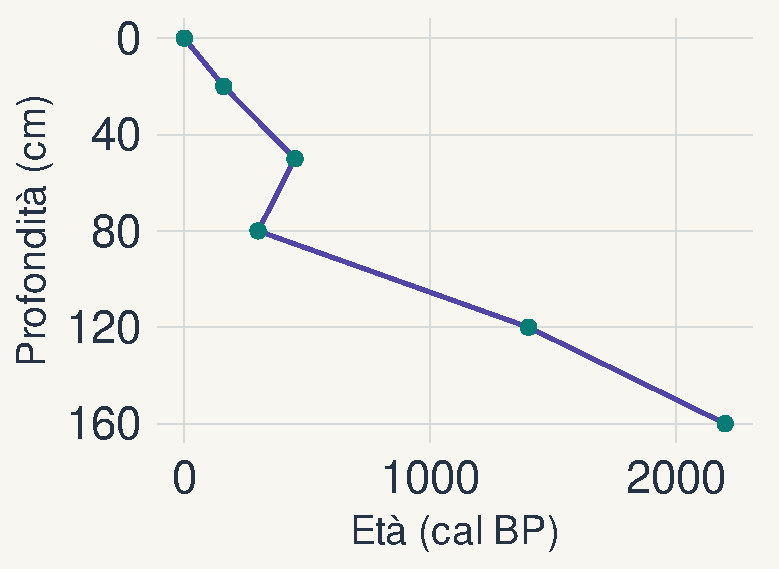
\includegraphics[width=\linewidth,height=6.15cm,keepaspectratio]{Figure/F08.pdf}\par}
\PSmall{Una sola ancora modificata produce un tratto cronologicamente invertito. La figura conserva l’ordine delle profondità.}
}};
\node[anchor=north west,inner sep=0] at([xshift=10.85cm,yshift=-2.12cm]current page.north west){\Colonna{8.16cm}{\PBody{Sostituendo in una copia l’età a ottanta centimetri con trecento anni, si introduce un’inversione fra cinquanta e ottanta centimetri. Il controllo individua il segmento nel quale l’età diminuisce con la profondità, mentre la spiegazione può richiedere un esame di errore analitico, rimaneggiamento, disturbo o associazione errata. Eliminare l’ancora soltanto perché ostacola la monotonicità trasferirebbe nel risultato una scelta non documentata. Eventuali esclusioni devono conservare il dato originario, la motivazione e un confronto di sensibilità.}
\par\smallskip{\centering\adjustbox{max width=.98\linewidth}{$\displaystyle \Delta t_i\le0\quad\Rightarrow\quad\text{verifica del segmento }i$}\par\smallskip}
}};
\end{tikzpicture}\end{frame}

\begin{frame}[plain]\hypertarget{slide44}{}
\bookmark[level=1,page=44]{Retta globale e variabilità dei tassi locali}
\begin{tikzpicture}[remember picture,overlay]
\PilotChrome{Retta globale e variabilità dei tassi locali}{DISCONTINUITÀ E SENSIBILITÀ DEL MODELLO}{44}{La flessibilità della curva deve essere giustificata dal processo e dalla capacità di previsione.}
\node[anchor=north west,inner sep=0] at([xshift=.96cm,yshift=-2.12cm]current page.north west){\Colonna{9.40cm}{{\centering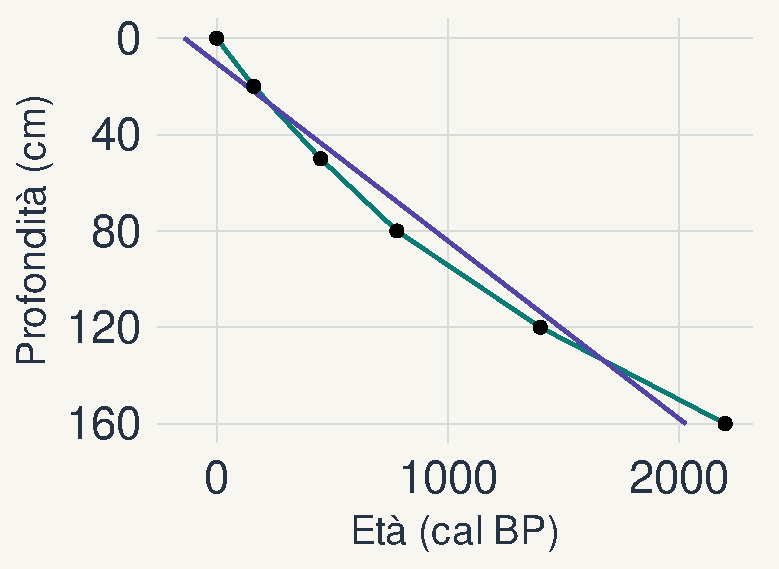
\includegraphics[width=\linewidth,height=6.15cm,keepaspectratio]{Figure/F09.pdf}\par}
\PSmall{$\beta_0$: intercetta; $\beta_1$: anni per cm; $\varepsilon$: scarto. Verde: interpolazione a tratti; viola: retta sulle sei ancore.}
}};
\node[anchor=north west,inner sep=0] at([xshift=10.85cm,yshift=-2.12cm]current page.north west){\Colonna{8.16cm}{\PBody{Una regressione lineare età–profondità assume un unico rapporto medio fra le due coordinate, mentre l’interpolazione a tratti consente cambiamenti di pendenza in corrispondenza delle ancore. La retta può avere residui anche quando la successione è monotona, poiché i tassi apparenti variano. L’interpolatore attraversa invece tutte le ancore per costruzione, cosicché il suo errore di adattamento nullo non dimostra migliore previsione. La scelta deve essere confrontata con il processo deposizionale, con la qualità delle ancore e con controlli esterni o di sensibilità.}
\par\smallskip{\centering\adjustbox{max width=.98\linewidth}{$\displaystyle t(z)=\beta_0+\beta_1z+\varepsilon$}\par\smallskip}
}};
\end{tikzpicture}\end{frame}

\begin{frame}[plain]\hypertarget{slide45}{}
\bookmark[level=1,page=45]{Esclusione di un’ancora interna e sensibilità locale}
\begin{tikzpicture}[remember picture,overlay]
\PilotChrome{Esclusione di un’ancora interna e sensibilità locale}{DISCONTINUITÀ E SENSIBILITÀ DEL MODELLO}{45}{La sensibilità a un’ancora va interpretata nel contesto della successione e del modello.}
\node[anchor=north west,inner sep=0] at([xshift=.96cm,yshift=-2.12cm]current page.north west){\Colonna{9.40cm}{{\centering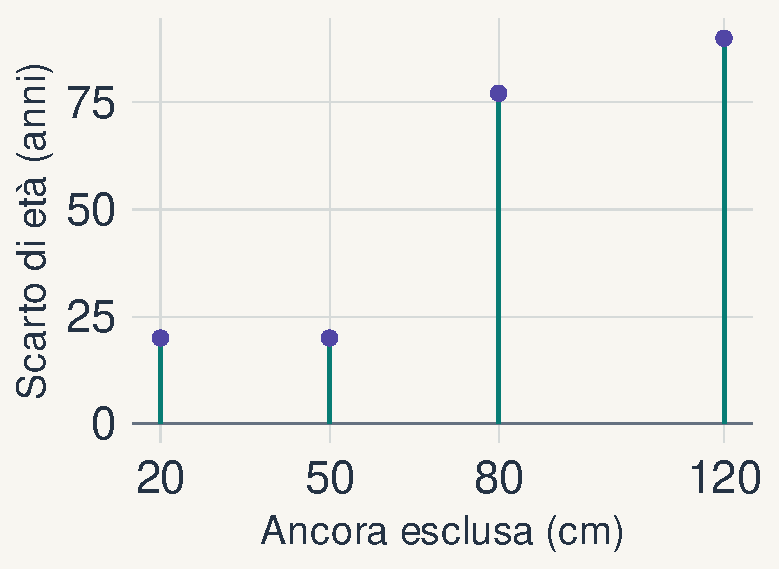
\includegraphics[width=\linewidth,height=6.15cm,keepaspectratio]{Figure/F10.pdf}\par}
\PSmall{Scarti delle quattro ancore interne dopo l’esclusione individuale. Il segno è previsto meno osservato.}
}};
\node[anchor=north west,inner sep=0] at([xshift=10.85cm,yshift=-2.12cm]current page.north west){\Colonna{8.16cm}{\PBody{Si elimina un’ancora interna alla volta e si stima la sua età mediante le ancore rimaste. Gli estremi vengono conservati, perché la loro esclusione richiederebbe estrapolazione. Gli scarti risultanti misurano quanto la ricostruzione locale dipenda dall’ancora omessa, senza riprodurre l’acquisizione di nuove datazioni indipendenti. Uno scarto ampio può segnalare una variazione reale del tasso, oltre a un possibile problema della misura. La verifica deve quindi orientare l’approfondimento e non diventare una regola automatica di eliminazione.}
\par\smallskip{\centering\adjustbox{max width=.98\linewidth}{$\displaystyle e_{(-i)}=\widehat t_{(-i)}(z_i)-t_i,\qquad i=2,\ldots,5$}\par\smallskip}
}};
\end{tikzpicture}\end{frame}

\begin{frame}[plain]\hypertarget{slide46}{}
\bookmark[level=1,page=46]{Una differenza negativa segnala un’inversione}
\begin{tikzpicture}[remember picture,overlay]
\PilotChrome{Una differenza negativa segnala un’inversione}{DISCONTINUITÀ E SENSIBILITÀ DEL MODELLO}{46}{Fra 50 e 80 cm la differenza di età vale –150 anni.}
\node[anchor=north west,inner sep=0] at([xshift=.96cm,yshift=-2.12cm]current page.north west){\Colonna{9.40cm}{\PLabel{Risultati del caso R6}
{\fontsize{10.2}{12.8}\selectfont\begin{tabular}{@{}>{\raggedright\arraybackslash}p{0.52\linewidth}@{\hspace{.13cm}}>{\raggedright\arraybackslash}p{0.39\linewidth}@{}}\toprule Grandezza & Valore\\[2.3pt]
\midrule 
Da (cm) & 50\\[2.3pt]
A (cm) & 80\\[2.3pt]
$\Delta$ anni & -150\\[2.3pt]
\bottomrule\end{tabular}\par}
}};
\node[anchor=north west,inner sep=0] at([xshift=10.85cm,yshift=-2.12cm]current page.north west){\Colonna{8.16cm}{\PBody{Per quale coppia di profondità il modello perturbato procede verso età più recenti andando in profondità?}
\vspace{.4cm}\PInfo{Fra 50 e 80 cm la differenza di età vale –150 anni. Si conserva la coppia originale per esaminare l’anomalia e la sua interpretazione stratigrafica.}
}};
\node[anchor=north east,inner sep=0] at([xshift=17.1cm,yshift=-12.04cm]current page.north west){\fontsize{7.7}{9}\selectfont \href{https://github.com/marzione00/Lab_Geo/blob/649f7cc577b96bd1044d81e78a2f530813e4f96b/materiali/laboratori/M13/M13_N14.R}{\color{Classical}\bfseries Script R · M13\_N14}};
\end{tikzpicture}\end{frame}

\begin{frame}[plain]\hypertarget{slide47}{}
\bookmark[level=1,page=47]{Togliere un’ancora misura la sensibilità locale}
\begin{tikzpicture}[remember picture,overlay]
\PilotChrome{Togliere un’ancora misura la sensibilità locale}{DISCONTINUITÀ E SENSIBILITÀ DEL MODELLO}{47}{L’errore è calcolato al livello escluso.}
\node[anchor=north west,inner sep=0] at([xshift=.96cm,yshift=-2.12cm]current page.north west){\Colonna{9.40cm}{\PLabel{Risultati del caso R6}
{\fontsize{10.2}{12.8}\selectfont\begin{tabular}{@{}>{\raggedright\arraybackslash}p{0.22\linewidth}@{\hspace{.13cm}}>{\raggedright\arraybackslash}p{0.22\linewidth}@{\hspace{.13cm}}>{\raggedright\arraybackslash}p{0.22\linewidth}@{\hspace{.13cm}}>{\raggedright\arraybackslash}p{0.23\linewidth}@{}}\toprule Profondità (cm) & osservata & prevista & errore\\[2.3pt]
\midrule 
20 & 160 & 180 & 20\\[2.3pt]
50 & 450 & 470 & 20\\[2.3pt]
80 & 780 & 857,14 & 77,143\\[2.3pt]
120 & 1400 & 1490 & 90\\[2.3pt]
\bottomrule\end{tabular}\par}
}};
\node[anchor=north west,inner sep=0] at([xshift=10.85cm,yshift=-2.12cm]current page.north west){\Colonna{8.16cm}{\PBody{Quanto si sbaglia nel ricostruire un livello interno usando solo le due ancore vicine?}
\vspace{.4cm}\PInfo{L’errore è calcolato al livello escluso. Un valore elevato segnala un tratto sensibile alla posizione di quell’ancora e merita attenzione nel modello.}
}};
\node[anchor=north east,inner sep=0] at([xshift=17.1cm,yshift=-12.04cm]current page.north west){\fontsize{7.7}{9}\selectfont \href{https://github.com/marzione00/Lab_Geo/blob/649f7cc577b96bd1044d81e78a2f530813e4f96b/materiali/laboratori/M13/M13_N16.R}{\color{Classical}\bfseries Script R · M13\_N16}};
\end{tikzpicture}\end{frame}

\begin{frame}[plain]\hypertarget{slide48}{}
\bookmark[level=1,page=48]{Discontinuità e sensibilità della cronologia}
\begin{tikzpicture}[remember picture,overlay]
\PilotChrome{Discontinuità e sensibilità della cronologia}{DISCONTINUITÀ E SENSIBILITÀ DEL MODELLO}{48}{Rappresentare un intervallo temporale privo di sedimentazione.}
\node[anchor=north west,inner sep=0] at([xshift=.96cm,yshift=-2.12cm]current page.north west){\Colonna{9.40cm}{{\centering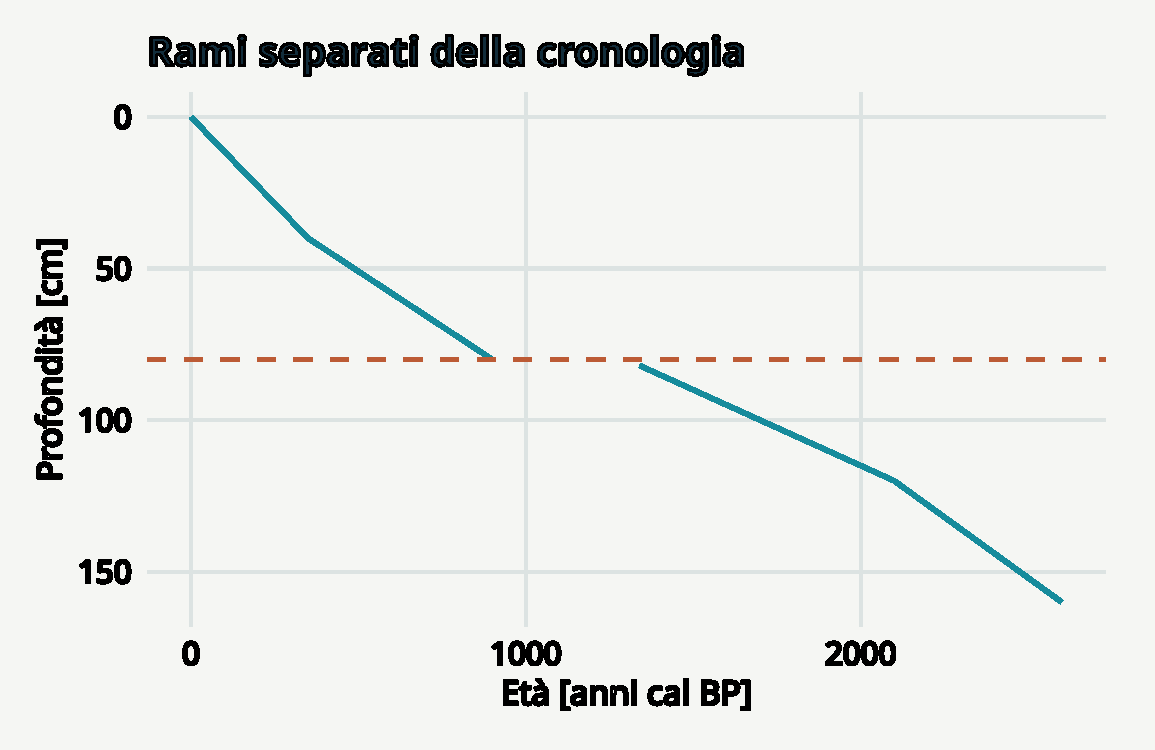
\includegraphics[width=\linewidth,height=6.0cm,keepaspectratio]{Esperimenti/m13-hiatus-A.pdf}\par}
\PSmall{Durata dello hiatus [anni]: 400. Seme: 17.}
}};
\node[anchor=north west,inner sep=0] at([xshift=10.85cm,yshift=-2.12cm]current page.north west){\Colonna{8.16cm}{\PLabel{Scenario A · simulazione}
\PBody{Uno hiatus rappresenta un intervallo temporale privo di sedimentazione conservata nel modello. L’esperimento aggiunge una durata controllabile alle età situate al di sotto di ottanta centimetri, lasciando invariata la cronologia della porzione superiore. I due rami vengono disegnati separatamente affinché una linea continua non suggerisca accumulo attraverso l’intervallo mancante.}
\par\smallskip{\centering\adjustbox{max width=.98\linewidth}{$\displaystyle t_H(z)=t(z)+H\mathbf1(z>80)$}\par\smallskip}
\PSmall{t(z) è la cronologia di base, H la durata dello hiatus e $\mathbf{1}(z>80)$ l’indicatore dei livelli più profondi di ottanta centimetri. Il ramo superiore include il livello di ottanta centimetri secondo la convenzione del codice.}
}};
\node[anchor=north east,inner sep=0] at([xshift=17.1cm,yshift=-12.04cm]current page.north west){\fontsize{7.7}{9}\selectfont \href{https://marzione00.github.io/Lab_Geo/\#laboratorio/m13-hiatus}{\color{Classical}\bfseries Apri il laboratorio · m13-hiatus}};
\end{tikzpicture}\end{frame}

\begin{frame}[plain]\hypertarget{slide49}{}
\bookmark[level=1,page=49]{Confronto | Discontinuità e sensibilità della cronologia}
\begin{tikzpicture}[remember picture,overlay]
\PilotChrome{Confronto | Discontinuità e sensibilità della cronologia}{DISCONTINUITÀ E SENSIBILITÀ DEL MODELLO}{49}{Lo hiatus produce un salto nella funzione età–profondità e richiede rami distinti nel disegno.}
\node[anchor=north west,inner sep=0] at([xshift=.96cm,yshift=-2.12cm]current page.north west){\Colonna{9.40cm}{{\centering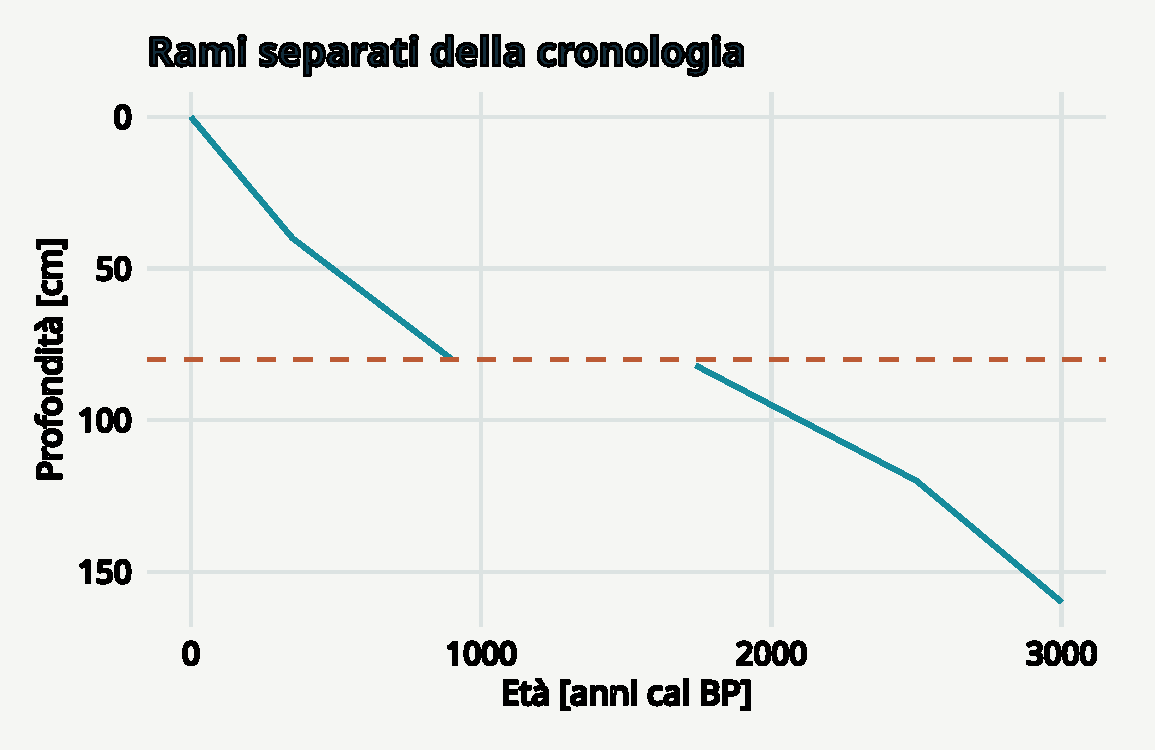
\includegraphics[width=\linewidth,height=5.6cm,keepaspectratio]{Esperimenti/m13-hiatus-B.pdf}\par}
\PSmall{Durata dello hiatus [anni]: 400 $\to$ 800. Tutti gli altri parametri e il seme sono fissi.}
}};
\node[anchor=north west,inner sep=0] at([xshift=10.85cm,yshift=-2.12cm]current page.north west){\Colonna{8.16cm}{\PLabel{Confronto fra gli scenari}
{\fontsize{10.2}{12.8}\selectfont\begin{tabular}{@{}>{\raggedright\arraybackslash}p{0.48\linewidth}@{\hspace{.13cm}}>{\raggedright\arraybackslash}p{0.224\linewidth}@{\hspace{.13cm}}>{\raggedright\arraybackslash}p{0.224\linewidth}@{}}\toprule Grandezza & A & B\\[2.3pt]
\midrule 
Salto cronologico [anni] & 400 & 800\\[2.3pt]
Età a 120 cm & 2100 & 2500\\[2.3pt]
\bottomrule\end{tabular}\par}
\vspace{.25cm}\PBody{Aumentando la lacuna di 400 anni, anche l’età a 120 cm aumenta di 400 anni. Sopra il limite il modello resta ancorato agli stessi livelli.}
}};
\node[anchor=north east,inner sep=0] at([xshift=17.1cm,yshift=-12.04cm]current page.north west){\fontsize{7.7}{9}\selectfont \href{https://marzione00.github.io/Lab_Geo/\#laboratorio/m13-hiatus}{\color{Classical}\bfseries Apri il laboratorio · m13-hiatus}};
\end{tikzpicture}\end{frame}

\begin{frame}[plain]\hypertarget{slide50}{}
\bookmark[level=0,page=50]{Pendenze, durate ed eventi}
\bookmark[level=1,page=50]{La durata usa due età della stessa cronologia}
\begin{tikzpicture}[remember picture,overlay]
\PilotChrome{La durata usa due età della stessa cronologia}{PENDENZE, DURATE ED EVENTI}{50}{Calcola la durata prima di riassumere la distribuzione degli scenari.}
\node[anchor=north west,inner sep=0] at([xshift=.96cm,yshift=-2.12cm]current page.north west){\Colonna{9.40cm}{\PLabel{Domanda}
\PBody{A 60 e 100 cm vogliamo stimare la durata di deposizione. Interrogare la stessa curva nei due punti preserva la dipendenza fra le età.}
\vspace{.35cm}\PLabel{Interpretazione}
\PBody{I livelli valgono 560 e 1090 anni cal BP. La loro differenza è 530 anni. Con scenari incerti si ripete la sottrazione dentro ogni singolo scenario.}
}};
\node[anchor=north west,inner sep=0] at([xshift=10.85cm,yshift=-2.12cm]current page.north west){\Colonna{8.16cm}{\begin{tcolorbox}[enhanced,arc=1.7mm,boxrule=.6pt,colback=white,colframe=Classical!60!Navy,colbacktitle=Navy,coltitle=white,fonttitle=\bfseries\small,title={R · calcolo riproducibile},left=1.7mm,right=1.3mm,top=1.1mm,bottom=1.1mm,before skip=1mm,after skip=1.0mm]\lstinputlisting[style=GeoR,language=R]{Codice/capitolo-06.R}\end{tcolorbox}
\PLabel{Risultato in R}
\begin{tcolorbox}[colback=GeoTint,colframe=Rule,boxrule=.5pt,arc=1.4mm,left=2mm,right=1mm,top=1mm,bottom=1mm]{\fontsize{9}{12}\selectfont\ttfamily \mbox{durata\ }\\\mbox{\ \ \ 560\ \ \ 1090\ \ \ \ 530}}\end{tcolorbox}}};
\end{tikzpicture}\end{frame}

\begin{frame}[plain]\hypertarget{slide51}{}
\bookmark[level=1,page=51]{Derivata del proxy e cambiamento di scala}
\begin{tikzpicture}[remember picture,overlay]
\PilotChrome{Derivata del proxy e cambiamento di scala}{PENDENZE, DURATE ED EVENTI}{51}{La trasformazione dell’asse cambia l’unità e l’interpretazione della variazione.}
\node[anchor=north west,inner sep=0] at([xshift=.96cm,yshift=-2.12cm]current page.north west){\Colonna{9.40cm}{{\centering\resizebox{.97\linewidth}{!}{\begin{tikzpicture}[x=1cm,y=-.87cm,every node/.style={font=\fontsize{12.2}{15}\selectfont,text=Ink},arr/.style={-{Stealth[length=2mm]},line width=.8pt,draw=Classical}]\path[use as bounding box] (0,0) rectangle (7.45,6.2);
\draw[draw=Classical,fill=Classical!8,rounded corners=2pt,line width=.7pt] (0.4,1.3) rectangle (2.9,3.4);
\node[anchor=center,text=Ink,font=\fontsize{16}{15}\selectfont] at (1.65,2.35) {$\mathrm dy/\mathrm dz$};
\draw[arr,draw=Quantum] (3.1,2.35)--(4.1,2.35);
\node[anchor=center,text=Ink,font=\fontsize{11}{15}\selectfont] at (3.6,1.4) {× r(z)};
\draw[draw=Quantum,fill=Quantum!8,rounded corners=2pt,line width=.7pt] (4.3,1.3) rectangle (6.8,3.4);
\node[anchor=center,text=Ink,font=\fontsize{16}{15}\selectfont] at (5.55,2.35) {$\mathrm dy/\mathrm dt$};
\node[anchor=center,text=Ink,font=\fontsize{12.2}{15}\selectfont,text width=6.7cm,align=center] at (3.7,4.7) {Il tasso locale collega le due unità.};
\node[anchor=center,text=Ink,font=\fontsize{10.8}{15}\selectfont,text width=6.8cm,align=center] at (3.7,5.7) {La relazione vale nei tratti regolari della cronologia.};

\end{tikzpicture}}\par}
\PSmall{y: proxy in u.a.; z: profondità in cm; t: età in anni; r(z): tasso in cm/anno. La derivata temporale è in u.a./anno.}
}};
\node[anchor=north west,inner sep=0] at([xshift=10.85cm,yshift=-2.12cm]current page.north west){\Colonna{8.16cm}{\PBody{La variazione del proxy per centimetro descrive il cambiamento lungo lo spessore, mentre la variazione per anno dipende anche dalla cronologia. Dove le funzioni sono derivabili e il tasso è positivo, la regola della catena collega le due derivate tramite il tasso locale di accumulo. Una conversione basata su un unico tasso medio è adeguata soltanto se la trasformazione dell’asse è coerente con tale approssimazione. Due regressioni globali sui diversi assi possono quindi restituire pendenze che non si ottengono mediante una semplice riscalatura costante.}
\par\smallskip{\centering\adjustbox{max width=.98\linewidth}{$\displaystyle \frac{\mathrm dy}{\mathrm dt}=\frac{\mathrm dy}{\mathrm dz}\frac{\mathrm dz}{\mathrm dt}=r(z)\frac{\mathrm dy}{\mathrm dz}$}\par\smallskip}
}};
\end{tikzpicture}\end{frame}

\begin{frame}[plain]\hypertarget{slide52}{}
\bookmark[level=1,page=52]{Durata di un intervallo e covarianza condivisa}
\begin{tikzpicture}[remember picture,overlay]
\PilotChrome{Durata di un intervallo e covarianza condivisa}{PENDENZE, DURATE ED EVENTI}{52}{Le quantità derivate da una cronologia devono conservare la struttura congiunta delle età.}
\node[anchor=north west,inner sep=0] at([xshift=.96cm,yshift=-2.12cm]current page.north west){\Colonna{9.40cm}{\PLabel{Metodo}
\PBody{La durata fra sessanta e cento centimetri si calcola sottraendo le due età all’interno dello stesso scenario. Le età condividono l’ancora a ottanta centimetri, per cui la loro covarianza entra nella varianza della differenza. Sottrarre quantili marginali costruirebbe una quantità diversa dai quantili della durata e perderebbe l’abbinamento fra scenari. Prima del condizionamento, la deviazione standard analitica è circa 48,94 anni; il codice verifica l’equivalenza delle forme matriciale ed espansa.}
}};
\node[anchor=north west,inner sep=0] at([xshift=10.85cm,yshift=-2.12cm]current page.north west){\Colonna{8.16cm}{\PLabel{Formalismo}
\par\smallskip{\centering\adjustbox{max width=.98\linewidth}{$\displaystyle D=T_2-T_1,\quad T_1=T(60),\ T_2=T(100)$}\par\smallskip}

\par\smallskip{\centering\adjustbox{max width=.98\linewidth}{$\displaystyle \operatorname{Var}(D)=\sigma_1^2+\sigma_2^2-2\sigma_{12}$}\par\smallskip}
\PLabel{Interpretazione}
\PBody{Nella formula, i termini quadratici indicano le varianze delle due età; il termine con indici 12 indica la loro covarianza. I pesi delle due profondità sono differenti: a 60 cm si combinano le ancore di 50 e 80 cm; a 100 cm si combinano quelle di 80 e 120 cm. La perturbazione dell’ancora condivisa entra in entrambe le età e viene parzialmente compensata nella differenza.}
}};
\end{tikzpicture}\end{frame}

\begin{frame}[plain]\hypertarget{slide53}{}
\bookmark[level=1,page=53]{Distribuzione degli scenari di durata}
\begin{tikzpicture}[remember picture,overlay]
\PilotChrome{Distribuzione degli scenari di durata}{PENDENZE, DURATE ED EVENTI}{53}{La durata viene derivata entro ciascuno scenario prima di riassumerne la distribuzione.}
\node[anchor=north west,inner sep=0] at([xshift=.96cm,yshift=-2.12cm]current page.north west){\Colonna{9.40cm}{\begin{tcolorbox}[enhanced,arc=1.7mm,boxrule=.6pt,colback=white,colframe=Classical!60!Navy,colbacktitle=Navy,coltitle=white,fonttitle=\bfseries\small,title={R · procedura},left=1.7mm,right=1.3mm,top=1.1mm,bottom=1.1mm,before skip=1mm,after skip=1.0mm]\lstinputlisting[style=GeoR,language=R]{Codice/lettura-27.R}\end{tcolorbox}
}};
\node[anchor=north west,inner sep=0] at([xshift=10.85cm,yshift=-2.12cm]current page.north west){\Colonna{8.16cm}{\PBody{La cronologia di base attribuisce 530 anni all’intervallo fra sessanta e cento centimetri. Negli scenari inclusi, la mediana è circa 529,7 anni e i quantili al 2,5\% e 97,5\% sono circa 433,0 e 630,5 anni. Il frammento ricostruisce la differenza per ciascun vettore di ancore, preservando la dipendenza richiesta. La distribuzione descrive soltanto le perturbazioni adottate e la regola lineare, mentre un hiatus entro l’intervallo o un diverso modello di accumulo modificherebbero il significato e il valore della durata.}
}};
\end{tikzpicture}\end{frame}

\begin{frame}[plain]\hypertarget{slide54}{}
\bookmark[level=1,page=54]{Confronto grafico delle durate ricostruite}
\begin{tikzpicture}[remember picture,overlay]
\PilotChrome{Confronto grafico delle durate ricostruite}{PENDENZE, DURATE ED EVENTI}{54}{L’incertezza di una durata dipende dalla collocazione delle ancore oltre che dall’ampiezza dell’intervallo.}
\node[anchor=north west,inner sep=0] at([xshift=.96cm,yshift=-2.12cm]current page.north west){\Colonna{9.40cm}{{\centering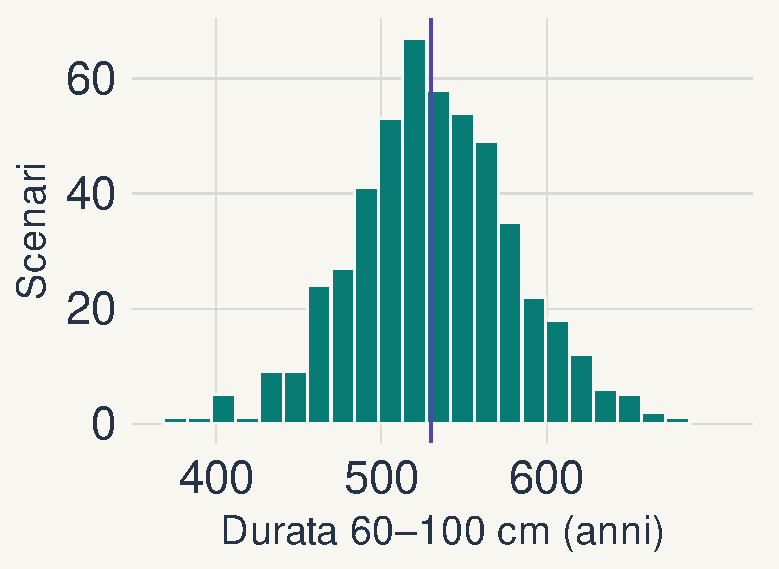
\includegraphics[width=\linewidth,height=6.15cm,keepaspectratio]{Figure/F11.pdf}\par}
\PSmall{Durata fra 60 e 100 centimetri nei cinquecento scenari; la linea viola indica i 530 anni della cronologia di base.}
}};
\node[anchor=north west,inner sep=0] at([xshift=10.85cm,yshift=-2.12cm]current page.north west){\Colonna{8.16cm}{\PBody{La distribuzione delle durate permette di distinguere il valore della cronologia di base dalla variabilità prodotta dalle ancore. La concentrazione degli scenari attorno a cinquecentotrenta anni riguarda l’intervallo selezionato e le deviazioni standard dichiarate. Intervalli con combinazioni diverse di ancore possono mostrare un’incertezza differente anche a parità di durata media. La lettura deve quindi collegare la forma dell’istogramma ai pesi dell’interpolazione, alla covarianza condivisa e alle fonti di variabilità che il modello ha lasciato fuori.}
}};
\end{tikzpicture}\end{frame}

\begin{frame}[plain]\hypertarget{slide55}{}
\bookmark[level=1,page=55]{Collocazione del massimo osservato del proxy}
\begin{tikzpicture}[remember picture,overlay]
\PilotChrome{Collocazione del massimo osservato del proxy}{PENDENZE, DURATE ED EVENTI}{55}{La collocazione temporale di un evento eredita le ipotesi della cronologia e l’incertezza del proxy.}
\node[anchor=north west,inner sep=0] at([xshift=.96cm,yshift=-2.12cm]current page.north west){\Colonna{9.40cm}{{\centering\resizebox{.97\linewidth}{!}{\begin{tikzpicture}[x=1cm,y=-.87cm,every node/.style={font=\fontsize{12.2}{15}\selectfont,text=Ink},arr/.style={-{Stealth[length=2mm]},line width=.8pt,draw=Classical}]\path[use as bounding box] (0,0) rectangle (7.45,6.2);
\draw[draw=Classical,fill=Classical!8,rounded corners=2pt,line width=.7pt] (0.5,0.8) rectangle (6.9,2);
\node[anchor=center,text=Ink,font=\fontsize{12.2}{15}\selectfont,text width=6cm,align=center] at (3.7,1.4) {Una misura: massimo a 160 cm};
\draw[arr,draw=Classical] (2.1,2.2)--(2.1,3.1);
\draw[arr,draw=Quantum] (5.3,2.2)--(5.3,3.1);
\draw[draw=Classical,fill=Classical!8,rounded corners=2pt,line width=.7pt] (0.5,3.3) rectangle (3.5,4.9);
\draw[draw=Quantum,fill=Quantum!8,rounded corners=2pt,line width=.7pt] (3.9,3.3) rectangle (6.9,4.9);
\node[anchor=center,text=Ink,font=\fontsize{11}{15}\selectfont,text width=2.6cm,align=center] at (2,4.1) {Base\par2200 cal BP};
\node[anchor=center,text=Ink,font=\fontsize{11}{15}\selectfont,text width=2.6cm,align=center] at (5.4,4.1) {Hiatus\par2600 cal BP};
\node[anchor=center,text=Ink,font=\fontsize{11}{15}\selectfont,text width=6.8cm,align=center] at (3.7,5.7) {Due modelli cronologici della stessa osservazione.};

\end{tikzpicture}}\par}
}};
\node[anchor=north west,inner sep=0] at([xshift=10.85cm,yshift=-2.12cm]current page.north west){\Colonna{8.16cm}{\PBody{Il massimo numerico del proxy sintetico si trova a 160 centimetri, al bordo inferiore dell’archivio. La cronologia di base gli assegna 2200 anni cal BP, mentre lo scenario con hiatus lo colloca a 2600 anni. La differenza deriva da due assunzioni cronologiche applicate alla stessa osservazione e non documenta uno spostamento reale dell’evento. La posizione al bordo richiede inoltre prudenza nell’identificare un picco completo, poiché la serie potrebbe proseguire oltre l’intervallo campionato. Rumore, risoluzione e significato del proxy devono accompagnare l’interpretazione geologica.}
\par\smallskip{\centering\adjustbox{max width=.98\linewidth}{$\displaystyle z_{\max}=\arg\max_{z_i}y_i,\qquad t_{\max}=t(z_{\max})$}\par\smallskip}
}};
\end{tikzpicture}\end{frame}

\begin{frame}[plain]\hypertarget{slide56}{}
\bookmark[level=1,page=56]{Le due estremità condividono l’incertezza cronologica}
\begin{tikzpicture}[remember picture,overlay]
\PilotChrome{Le due estremità condividono l’incertezza cronologica}{PENDENZE, DURATE ED EVENTI}{56}{I quantili sono calcolati dopo aver sottratto le età all’interno dello stesso scenario.}
\node[anchor=north west,inner sep=0] at([xshift=.96cm,yshift=-2.12cm]current page.north west){\Colonna{9.40cm}{\PLabel{Risultati del caso R6}
{\fontsize{10.2}{12.8}\selectfont\begin{tabular}{@{}>{\raggedright\arraybackslash}p{0.44\linewidth}@{\hspace{.13cm}}>{\raggedright\arraybackslash}p{0.48\linewidth}@{}}\toprule Probabilità & Durata (anni)\\[2.3pt]
\midrule 
0,025 & 433\\[2.3pt]
0,5 & 529,67\\[2.3pt]
0,975 & 630,49\\[2.3pt]
\bottomrule\end{tabular}\par}
}};
\node[anchor=north west,inner sep=0] at([xshift=10.85cm,yshift=-2.12cm]current page.north west){\Colonna{8.16cm}{\PBody{Quali durate risultano fra 60 e 100 cm nelle cronologie simulate?}
\vspace{.4cm}\PInfo{I quantili sono calcolati dopo aver sottratto le età all’interno dello stesso scenario. La media o la differenza di quantili marginali risponderebbero a domande diverse.}
}};
\node[anchor=north east,inner sep=0] at([xshift=17.1cm,yshift=-12.04cm]current page.north west){\fontsize{7.7}{9}\selectfont \href{https://github.com/marzione00/Lab_Geo/blob/649f7cc577b96bd1044d81e78a2f530813e4f96b/materiali/laboratori/M13/M13_N18.R}{\color{Classical}\bfseries Script R · M13\_N18}};
\end{tikzpicture}\end{frame}

\begin{frame}[plain]\hypertarget{slide57}{}
\bookmark[level=1,page=57]{Durate entro uno stesso scenario}
\begin{tikzpicture}[remember picture,overlay]
\PilotChrome{Durate entro uno stesso scenario}{PENDENZE, DURATE ED EVENTI}{57}{Propagare la covarianza nella durata fra due eventi.}
\node[anchor=north west,inner sep=0] at([xshift=.96cm,yshift=-2.12cm]current page.north west){\Colonna{9.40cm}{{\centering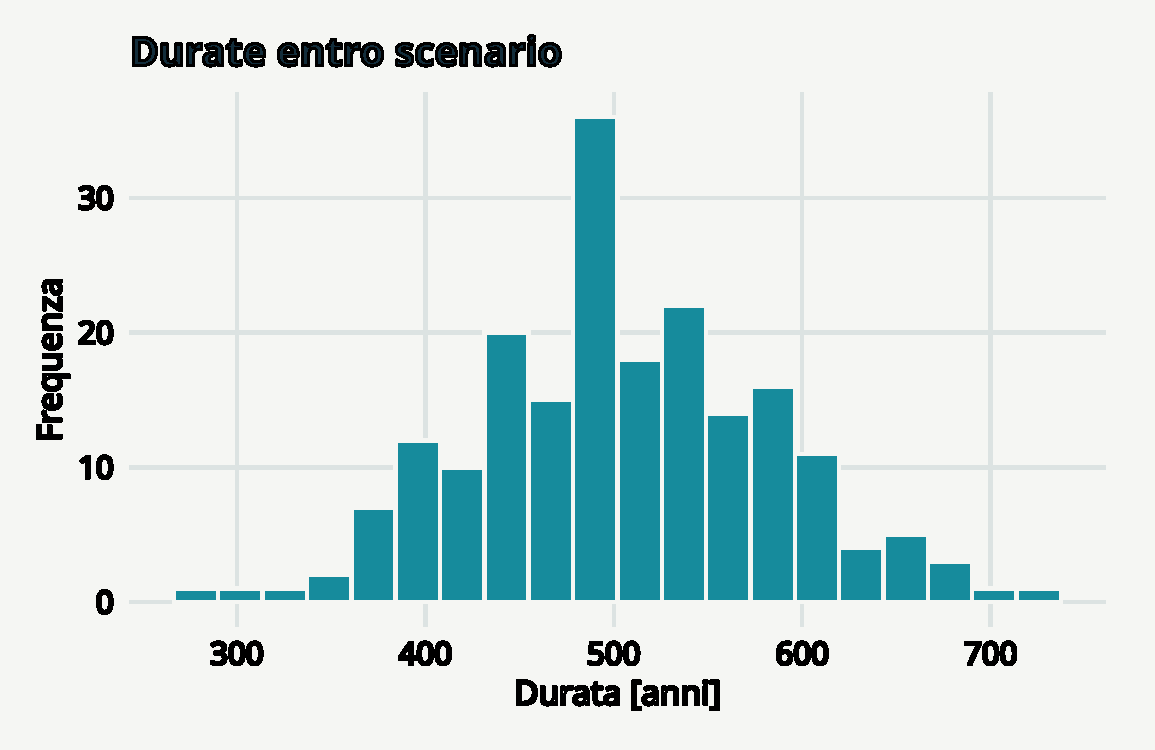
\includegraphics[width=\linewidth,height=6.0cm,keepaspectratio]{Esperimenti/m13-durate-A.pdf}\par}
\PSmall{Correlazione fra le età: 0,6. Seme: 17.}
}};
\node[anchor=north west,inner sep=0] at([xshift=10.85cm,yshift=-2.12cm]current page.north west){\Colonna{8.16cm}{\PLabel{Scenario A · simulazione}
\PBody{La durata fra due eventi si ottiene sottraendo le loro età entro la medesima configurazione cronologica. L’esperimento genera coppie di età gaussiane con dispersioni fissate e correlazione controllabile, dalle quali ricava una distribuzione di differenze. La deviazione standard simulata viene confrontata con quella ottenuta dalla formula analitica, rendendo verificabile la propagazione della covarianza.}
\par\smallskip{\centering\adjustbox{max width=.98\linewidth}{$\displaystyle \operatorname{Var}(T_2-T_1)=\sigma_1^2+\sigma_2^2-2\rho\sigma_1\sigma_2$}\par\smallskip}
\PSmall{$T_1$ e $T_2$ sono le età dei due eventi; $\sigma_1$ e $\sigma_2$ le loro deviazioni standard; $\rho$ la correlazione. La durata è $T_2-T_1$ e la covarianza è $\rho\sigma_1\sigma_2$.}
}};
\node[anchor=north east,inner sep=0] at([xshift=17.1cm,yshift=-12.04cm]current page.north west){\fontsize{7.7}{9}\selectfont \href{https://marzione00.github.io/Lab_Geo/\#laboratorio/m13-durate}{\color{Classical}\bfseries Apri il laboratorio · m13-durate}};
\end{tikzpicture}\end{frame}

\begin{frame}[plain]\hypertarget{slide58}{}
\bookmark[level=1,page=58]{Confronto | Durate entro uno stesso scenario}
\begin{tikzpicture}[remember picture,overlay]
\PilotChrome{Confronto | Durate entro uno stesso scenario}{PENDENZE, DURATE ED EVENTI}{58}{La durata va calcolata accoppiando le età appartenenti al medesimo scenario.}
\node[anchor=north west,inner sep=0] at([xshift=.96cm,yshift=-2.12cm]current page.north west){\Colonna{9.40cm}{{\centering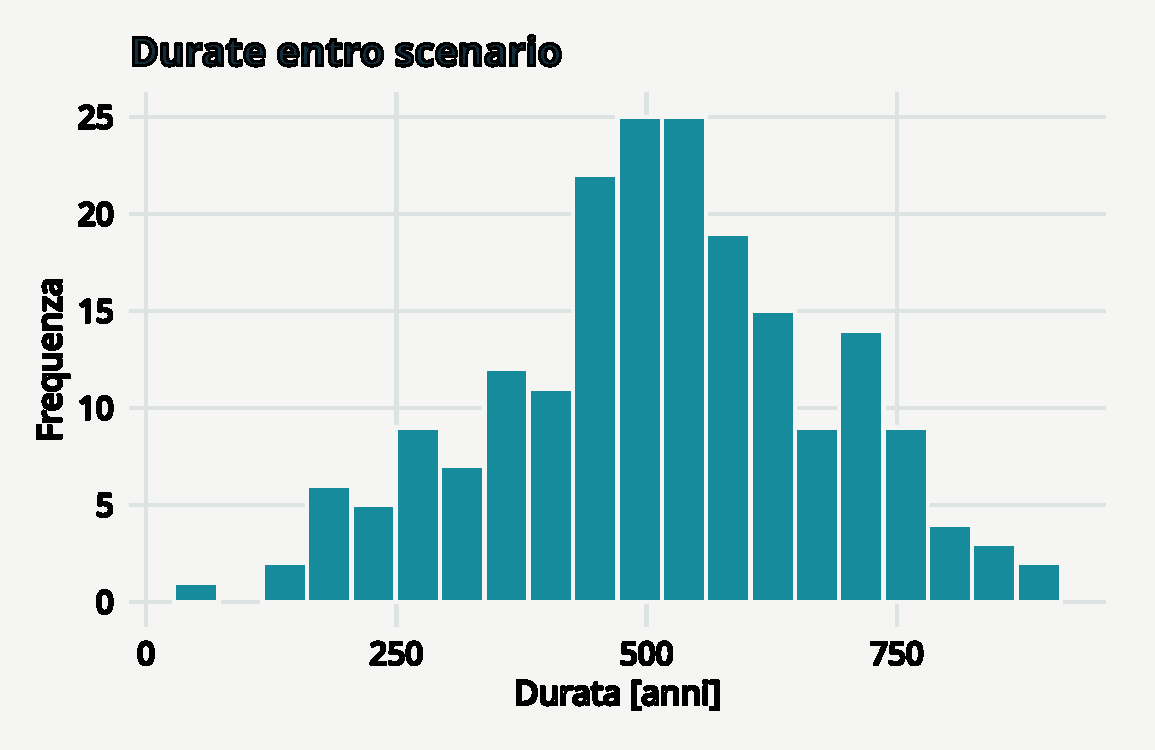
\includegraphics[width=\linewidth,height=5.6cm,keepaspectratio]{Esperimenti/m13-durate-B.pdf}\par}
\PSmall{Correlazione fra le età: 0,6 $\to$ -0,6. Tutti gli altri parametri e il seme sono fissi.}
}};
\node[anchor=north west,inner sep=0] at([xshift=10.85cm,yshift=-2.12cm]current page.north west){\Colonna{8.16cm}{\PLabel{Confronto fra gli scenari}
{\fontsize{10.2}{12.8}\selectfont\begin{tabular}{@{}>{\raggedright\arraybackslash}p{0.48\linewidth}@{\hspace{.13cm}}>{\raggedright\arraybackslash}p{0.224\linewidth}@{\hspace{.13cm}}>{\raggedright\arraybackslash}p{0.224\linewidth}@{}}\toprule Grandezza & A & B\\[2.3pt]
\midrule 
SD simulata [anni] & 79,6 & 165\\[2.3pt]
SD analitica [anni] & 82,5 & 161\\[2.3pt]
Durata media & 505 & 511\\[2.3pt]
\bottomrule\end{tabular}\par}
\vspace{.25cm}\PBody{Quando la correlazione passa da positiva a negativa, gli errori delle due età tendono a sommarsi nella differenza. La dispersione simulata cresce da circa 80 a 165 anni.}
}};
\node[anchor=north east,inner sep=0] at([xshift=17.1cm,yshift=-12.04cm]current page.north west){\fontsize{7.7}{9}\selectfont \href{https://marzione00.github.io/Lab_Geo/\#laboratorio/m13-durate}{\color{Classical}\bfseries Apri il laboratorio · m13-durate}};
\end{tikzpicture}\end{frame}

\begin{frame}[plain]\hypertarget{slide59}{}
\bookmark[level=0,page=59]{Consegna e studio autonomo}
\bookmark[level=1,page=59]{Il massimo osservato resta nello stesso campione}
\begin{tikzpicture}[remember picture,overlay]
\PilotChrome{Il massimo osservato resta nello stesso campione}{CONSEGNA E STUDIO AUTONOMO}{59}{Distingui posizione osservata, età modellata e risoluzione del prelievo.}
\node[anchor=north west,inner sep=0] at([xshift=.96cm,yshift=-2.12cm]current page.north west){\Colonna{9.40cm}{\PLabel{Domanda}
\PBody{Il massimo del proxy della carota sintetica è a 160 cm. Come cambia la sua datazione se si introduce la lacuna a 80 cm?}
\vspace{.35cm}\PLabel{Interpretazione}
\PBody{Il campione resta quello a 160 cm. Il suo massimo passa da 2200 a 2600 anni cal BP. Un picco situato fra due campioni potrebbe sfuggire a entrambi i modelli.}
}};
\node[anchor=north west,inner sep=0] at([xshift=10.85cm,yshift=-2.12cm]current page.north west){\Colonna{8.16cm}{\begin{tcolorbox}[enhanced,arc=1.7mm,boxrule=.6pt,colback=white,colframe=Classical!60!Navy,colbacktitle=Navy,coltitle=white,fonttitle=\bfseries\small,title={R · calcolo riproducibile},left=1.7mm,right=1.3mm,top=1.1mm,bottom=1.1mm,before skip=1mm,after skip=1.0mm]\lstinputlisting[style=GeoR,language=R]{Codice/capitolo-07.R}\end{tcolorbox}
\PLabel{Risultato in R}
\begin{tcolorbox}[colback=GeoTint,colframe=Rule,boxrule=.5pt,arc=1.4mm,left=2mm,right=1mm,top=1mm,bottom=1mm]{\fontsize{9}{12}\selectfont\ttfamily \mbox{base\ con\_lacuna\ }\\\mbox{\ \ \ \ \ \ 2200\ \ \ \ \ \ \ 2600}}\end{tcolorbox}}};
\end{tikzpicture}\end{frame}

\begin{frame}[plain]\hypertarget{slide60}{}
\bookmark[level=1,page=60]{Metadati cronologici e percorso di laboratorio}
\begin{tikzpicture}[remember picture,overlay]
\PilotChrome{Metadati cronologici e percorso di laboratorio}{CONSEGNA E STUDIO AUTONOMO}{60}{La cronologia deve essere riproducibile come procedimento e interpretabile come insieme di ipotesi.}
\node[anchor=north west,inner sep=0] at([xshift=.96cm,yshift=-2.12cm]current page.north west){\Colonna{9.40cm}{{\centering\resizebox{.97\linewidth}{!}{\begin{tikzpicture}[x=1cm,y=-.87cm,every node/.style={font=\fontsize{12.2}{15}\selectfont,text=Ink},arr/.style={-{Stealth[length=2mm]},line width=.8pt,draw=Classical}]\path[use as bounding box] (0,0) rectangle (7.45,6.2);
\draw[draw=Classical,fill=Classical!8,rounded corners=2pt,line width=.7pt] (0.5,0.6) rectangle (6.9,1.9);
\node[anchor=center,text=Ink,font=\fontsize{12.2}{15}\selectfont,text width=6cm,align=center] at (3.7,1.25) {Ancore, materiali e metadati};
\draw[arr,draw=Classical] (3.7,2.1)--(3.7,2.6);
\draw[draw=Quantum,fill=Quantum!8,rounded corners=2pt,line width=.7pt] (0.5,2.8) rectangle (6.9,4.1);
\node[anchor=center,text=Ink,font=\fontsize{12.2}{15}\selectfont,text width=6cm,align=center] at (3.7,3.45) {Modello cronologico e scenari};
\draw[arr,draw=Classical] (3.7,4.3)--(3.7,4.8);
\node[anchor=center,text=Ink,font=\fontsize{11.5}{15}\selectfont,text width=6.7cm,align=center] at (3.7,5.4) {Età, durate e proxy con provenienza};

\end{tikzpicture}}\par}
}};
\node[anchor=north west,inner sep=0] at([xshift=10.85cm,yshift=-2.12cm]current page.north west){\Colonna{8.16cm}{\PBody{La consegna conserva ancore originali, unità di profondità, convenzione BP, metodo di interpolazione, dominio, scenari di incertezza e decisioni di esclusione. I laboratori N01–N07 sviluppano controlli e tassi; N08–N12 propagano gli scenari e trasformano il proxy; N13–N16 esaminano discontinuità e sensibilità; N17–N20 completano pendenze, durate ed esportazione. Per lo studio autonomo si raddoppino le deviazioni standard e si confrontino numero di scenari accettati, età a cento centimetri e durata dell’intervallo sessanta–cento centimetri, motivando le differenze osservate.}
}};
\end{tikzpicture}\end{frame}

\begin{frame}[plain]\hypertarget{slide61}{}
\bookmark[level=1,page=61]{Un massimo può essere vicino al bordo del record}
\begin{tikzpicture}[remember picture,overlay]
\PilotChrome{Un massimo può essere vicino al bordo del record}{CONSEGNA E STUDIO AUTONOMO}{61}{La posizione del massimo campionato è robusta rispetto alla trasformazione dell’asse.}
\node[anchor=north west,inner sep=0] at([xshift=.96cm,yshift=-2.12cm]current page.north west){\Colonna{9.40cm}{\PLabel{Risultati del caso R6}
{\fontsize{10.2}{12.8}\selectfont\begin{tabular}{@{}>{\raggedright\arraybackslash}p{0.52\linewidth}@{\hspace{.13cm}}>{\raggedright\arraybackslash}p{0.39\linewidth}@{}}\toprule Grandezza & Valore\\[2.3pt]
\midrule 
Profondità (cm) & 160\\[2.3pt]
proxy & 3,2377\\[2.3pt]
eta base & 2200\\[2.3pt]
eta hiatus & 2600\\[2.3pt]
\bottomrule\end{tabular}\par}
}};
\node[anchor=north west,inner sep=0] at([xshift=10.85cm,yshift=-2.12cm]current page.north west){\Colonna{8.16cm}{\PBody{Quale conclusione regge al confronto fra cronologia di base e cronologia con lacuna?}
\vspace{.4cm}\PInfo{La posizione del massimo campionato è robusta rispetto alla trasformazione dell’asse. La sua età cambia di 400 anni e il record termina proprio a quella profondità.}
}};
\node[anchor=north east,inner sep=0] at([xshift=17.1cm,yshift=-12.04cm]current page.north west){\fontsize{7.7}{9}\selectfont \href{https://github.com/marzione00/Lab_Geo/blob/649f7cc577b96bd1044d81e78a2f530813e4f96b/materiali/laboratori/M13/M13_N20.R}{\color{Classical}\bfseries Script R · M13\_N20}};
\end{tikzpicture}\end{frame}

\begin{frame}[plain]\hypertarget{slide62}{}
\bookmark[level=1,page=62]{Dal risultato alla relazione}
\begin{tikzpicture}[remember picture,overlay]
\PilotChrome{Dal risultato alla relazione}{SINTESI}{62}{Una conclusione cronologica riporta profondità, convenzione temporale, modello e sensibilità alle ancore.}
\node[anchor=north west,inner sep=0] at([xshift=.96cm,yshift=-2.12cm]current page.north west){\Colonna{9.40cm}{\PLabel{Domanda di partenza}
\PBody{Quando si è depositato il livello in cui il proxy raggiunge il massimo osservato?}
\PLabel{Risultato da discutere}
\PBody{Il massimo campionato è a 160 cm. La cronologia di base lo colloca a 2200 cal BP. Una lacuna di 400 anni a 80 cm lo colloca a 2600 cal BP.}
}};
\node[anchor=north west,inner sep=0] at([xshift=10.85cm,yshift=-2.12cm]current page.north west){\Colonna{8.16cm}{\PLabel{Limiti della conclusione}
\PBody{La posizione coincide con il bordo del record. Le età dipendono dal modello di accumulo e il prelievo ogni 2 cm limita la risoluzione del proxy.}
\vspace{.4cm}\href{https://marzione00.github.io/Lab_Geo/\#modulo-P08}{\color{Classical}\bfseries Prosegui · P08 · Collocare nel tempo il massimo di un proxy}}};
\end{tikzpicture}\end{frame}

\begin{frame}[plain]\hypertarget{slide63}{}
\bookmark[level=1,page=63]{Fonti, dati e codice per riprodurre le figure}
\begin{tikzpicture}[remember picture,overlay]
\PilotChrome{Fonti, dati e codice per riprodurre le figure}{RIFERIMENTI}{63}{I dataset della carota e del simulatore sono esempi distinti con ancore dichiarate.}
\node[anchor=north west,inner sep=0] at([xshift=.96cm,yshift=-2.12cm]current page.north west){\Colonna{9.40cm}{\PLabel{Materiali del corso}
\PBody{Il fascicolo deriva dal modulo M13 di GeoStat Lab e dai materiali didattici di Marzio De Corato. I dati del caso guida sono didattici. Le simulazioni A e B riportano il proprio seme.}
\href{https://github.com/marzione00/Lab_Geo/blob/649f7cc577b96bd1044d81e78a2f530813e4f96b/moduli/M13/README.md}{\color{Classical}\bfseries Scheda e documentazione originale}\par\smallskip \href{https://github.com/marzione00/Lab_Geo/blob/649f7cc577b96bd1044d81e78a2f530813e4f96b/materiali/R/M13_figure.R}{\color{Classical}\bfseries Script R delle figure del corso}}};
\node[anchor=north west,inner sep=0] at([xshift=10.85cm,yshift=-2.12cm]current page.north west){\Colonna{8.16cm}{\PLabel{Nell’archivio dei sorgenti}
\PBody{Codice contiene i frammenti delle pagine. Esperimenti comprende i due programmi R e i risultati di ciascun confronto. Diagrammi contiene i disegni TikZ modificabili. Scena conserva il modello Blender della copertina.}
\vspace{.4cm}\href{https://marzione00.github.io/Lab_Geo/\#modulo-M13}{\color{Classical}\bfseries Apri Strata su GeoStat Lab}}};
\end{tikzpicture}\end{frame}

\end{document}